\chapter{Vers une génération de rapports de biopsie automatique avec MyoQuant}
Avec \gls{impatient} et \gls{nlmyo} nous avons développé des outils capables de traiter et d'explorer les comptes-rendus de biopsies textuels, permettant ainsi une approche rétrospective de l'ensemble des patients connus à ce jour. Cependant, il est intéressant d'explorer aussi comment l'analyse d'images par \gls{ia} peut permettre de générer automatiquement des comptes-rendus de biopsies. Cette approche permettrait un gain de précision et de temps dans l'évaluation des biopsies. Tout d'abord un gain de temps, car une approche par \gls{ia} permettrait de détecter et de quantifier les marqueurs pathologiques sur des biopsies de grande résolution dans de multiples colorations de manière automatique, libérant ainsi le temps utilisé pour l'interprétation des coupes histologiques. Ensuite un gain de précision, car l'évaluation des biopsies par un expert humain n'est en général que qualitative. La description de phénotype se limite généralement à des adjectifs de quantité tels que "peu", "moyen" ou "beaucoup". Grâce à une approche de comptage par \gls{ia}, il est alors possible d'obtenir la quantité précise pour chaque marqueur évalué tel que le nombre de fibres présentant un noyau centralisé et ainsi de pouvoir établir des seuils pour une analyse plus approfondie.


Le stockage, la gestion et l'exploitation des images en microscopie de grande taille sont des problématiques pour lesquelles de nombreux outils ont été développés. Dans un effort d'uniformisation des formats et des interfaces, on peut notamment citer la plateforme OMERO (Open Microscopy Environment \cite{allan_omero_2012}). Cette plateforme cherche à unifier les scientifiques et les développeurs autour de procédures et de format standard de stockage et d'ajout de métadonnées pour les données expérimentales de microscopie. D'autre initiative telle que Cytomine (\cite{maree_collaborative_2016} ) a été développée pour permettre l'analyse collaborative d'images biomédicales. Cependant, encore aujourd'hui, ces outils de gestions des données d'imagerie ne sont pas largement répandus parmi les chercheurs. De plus pour la quantification d'images, il est souvent préféré et nécessaire de développer des scripts d'analyse taillés spécifique au besoin d'analyse du projet. Dans ce cadre-là, nous avons développé une série de méthodes génériques applicables pour l'analyse de biopsie du muscle.

\gls{myoquant}, l'outil présenté dans ce chapitre, est une suite de méthodes pour quantifier différents marqueurs histopathologiques dans les biopsies de \gls{mc}. \gls{myoquant} intègre à la fois des méthodes algorithmiques simples basées sur des modèles d'\gls{ia} généralistes en histologie comme CellPose (\cite{stringer_cellpose_2021}) et Stardist (\cite{weigert_star-convex_2020}), soit des méthodes basées sur des modèles \gls{ia} que nous avons développés à partir de nos données. Actuellement, \gls{myoquant} est capable de quantifier des marqueurs pathologiques dans trois des cinq colorations réalisées en routine lors du diagnostic des \gls{mc}: la centralisation des noyaux à la coloration \gls{he}, un déséquilibre dans le ratio des fibres de type 1 et 2 à la coloration ATPase et une répartition anormale des mitochondries dans les fibres musculaires à la coloration \gls{sdh}. Dans ce chapitre, nous allons voir comment ont été implémentés ces solutions de quantification automatique et des exemples d'application.

\begin{figure}[!ht]
 \centering
 
\includegraphics[width=0.66\textwidth]{figures/myoquant_logo.png}
 \caption[Logo MyoQuant]{\textbf{Logo de MyoQuant}. MyoQuant est un outil permettant de quantifier automatiquement des marqueurs pathologiques dans les biopsies musculaires. Cet outil open source est disponible en ligne de commande (\gls{myoquant}) et en version de démonstration en ligne (\gls{myoquant}-Streamlit). \url{https://github.com/lambda-science/MyoQuant}}
 \label{fig:myoquant_logo}
\end{figure}

\section{Analyse de la position des noyaux cellulaires}
Dans un premier temps, nous nous sommes intéressés à l'analyse de la position des noyaux cellulaires dans les fibres musculaires. Dans un muscle sain, les noyaux sont en général en périphérie des fibres, tandis que dans les muscles des patients atteints de \gls{mc} et particulièrement dans les \gls{cnm}, les noyaux peuvent être internalisés, voire centralisés. Par exemple, dans la figure \ref{fig:he_example}, on observe un nombre important de fibres ayant un noyau cellulaire internalisé (flèche noire). Nous avons dès lors développé une méthode pour compter automatiquement le nombre de fibres présentant un noyau internalisé.
\begin{figure}[!ht]
 \centering
 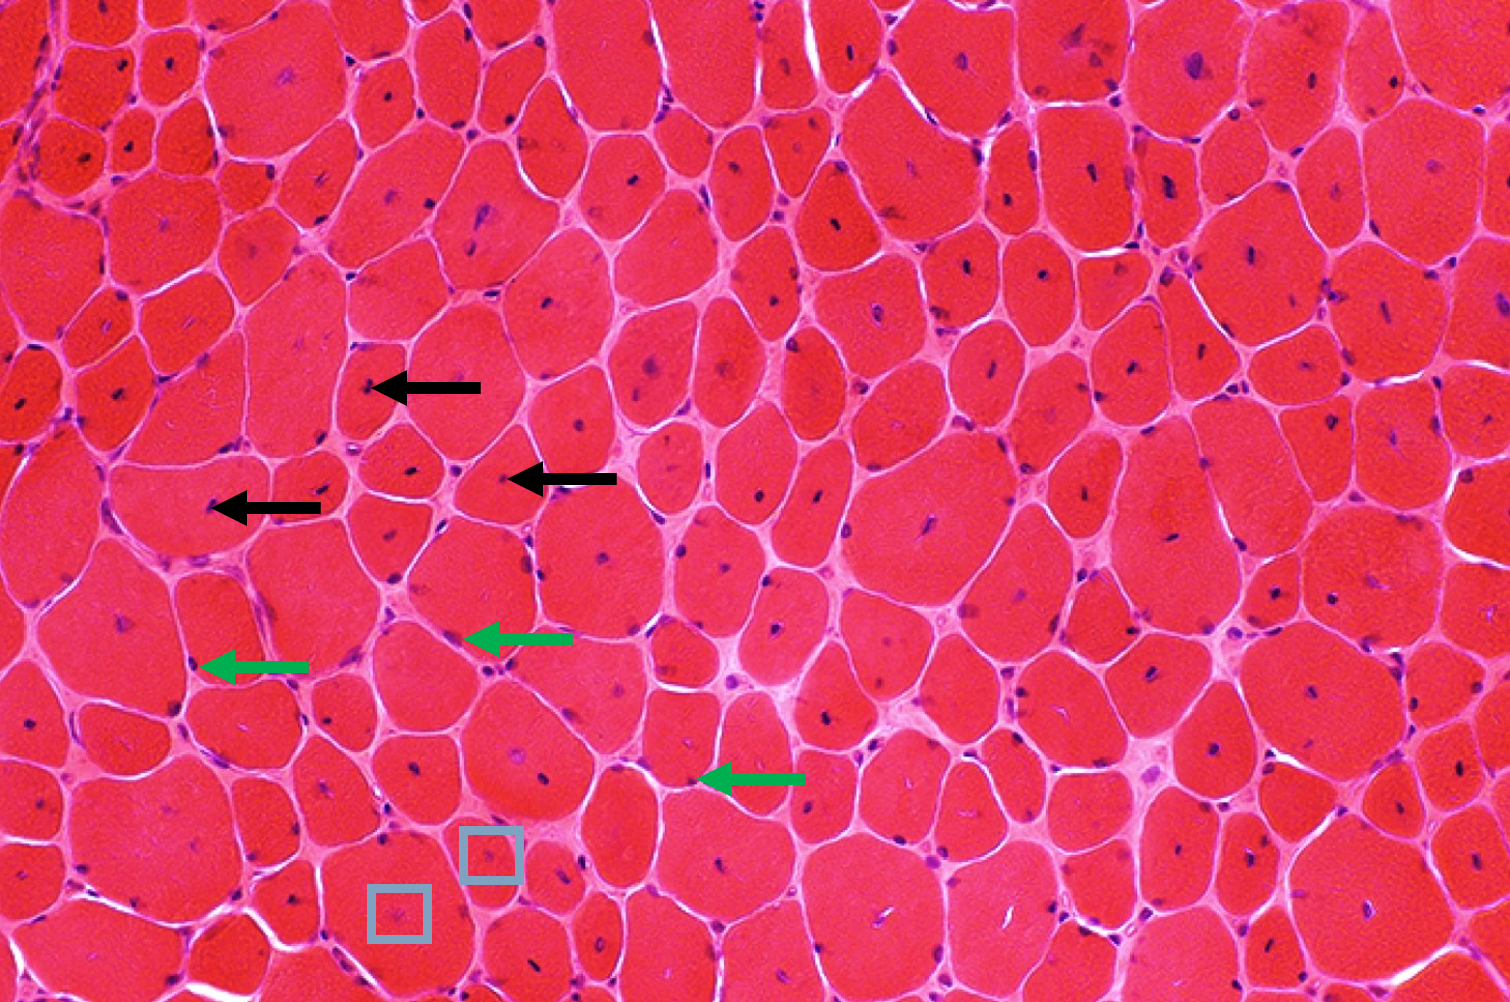
\includegraphics[width=0.8\textwidth]{figures/he_example.jpg}
 \caption[Exemple de biopsie musculaire à la coloration HE]{\textbf{Exemple de biopsie musculaire de CNM à la coloration HE }. On observe des fibres avec des noyaux centralisés (indiqués par des flèches noires) et des noyaux périphériques (flèches vertes). De plus, on observe des noyaux avec une faible intensité de marquage (carrés bleus).}
 \label{fig:he_example}
\end{figure}

\subsection{Algorithme de quantification}
Pour réaliser la quantification des noyaux centralisés, la première étape consiste à obtenir la position de toutes les fibres musculaires et de tous les noyaux de la coupe (segmentation). Pour cela, nous avons utilisé deux modèles d'\gls{ia} généralistes développés spécifiquement pour l'analyse de coupes histologiques: Cellpose et Stardist. Cellpose nous a permis de segmenter les fibres musculaires, tandis que Stardist nous a permis de segmenter les noyaux cellulaires. La figure \ref{fig:he_seg} présente les résultats de la segmentation de la biopsie présentée en figure \ref{fig:he_example}. On observe que globalement toutes les fibres musculaires sont bien segmentées, cependant concernant les noyaux cellulaires, certains sont trop peu colorés pour être reconnus par le modèle. C'est notamment le cas pour quelques noyaux centraux sur la gauche de la biopsie (indiqué par des carrés bleus), ce qui sera problématique lors de l'analyse des noyaux, car ils ne seront pas détectés par Stardist.
\begin{figure}[!ht]
 \centering
 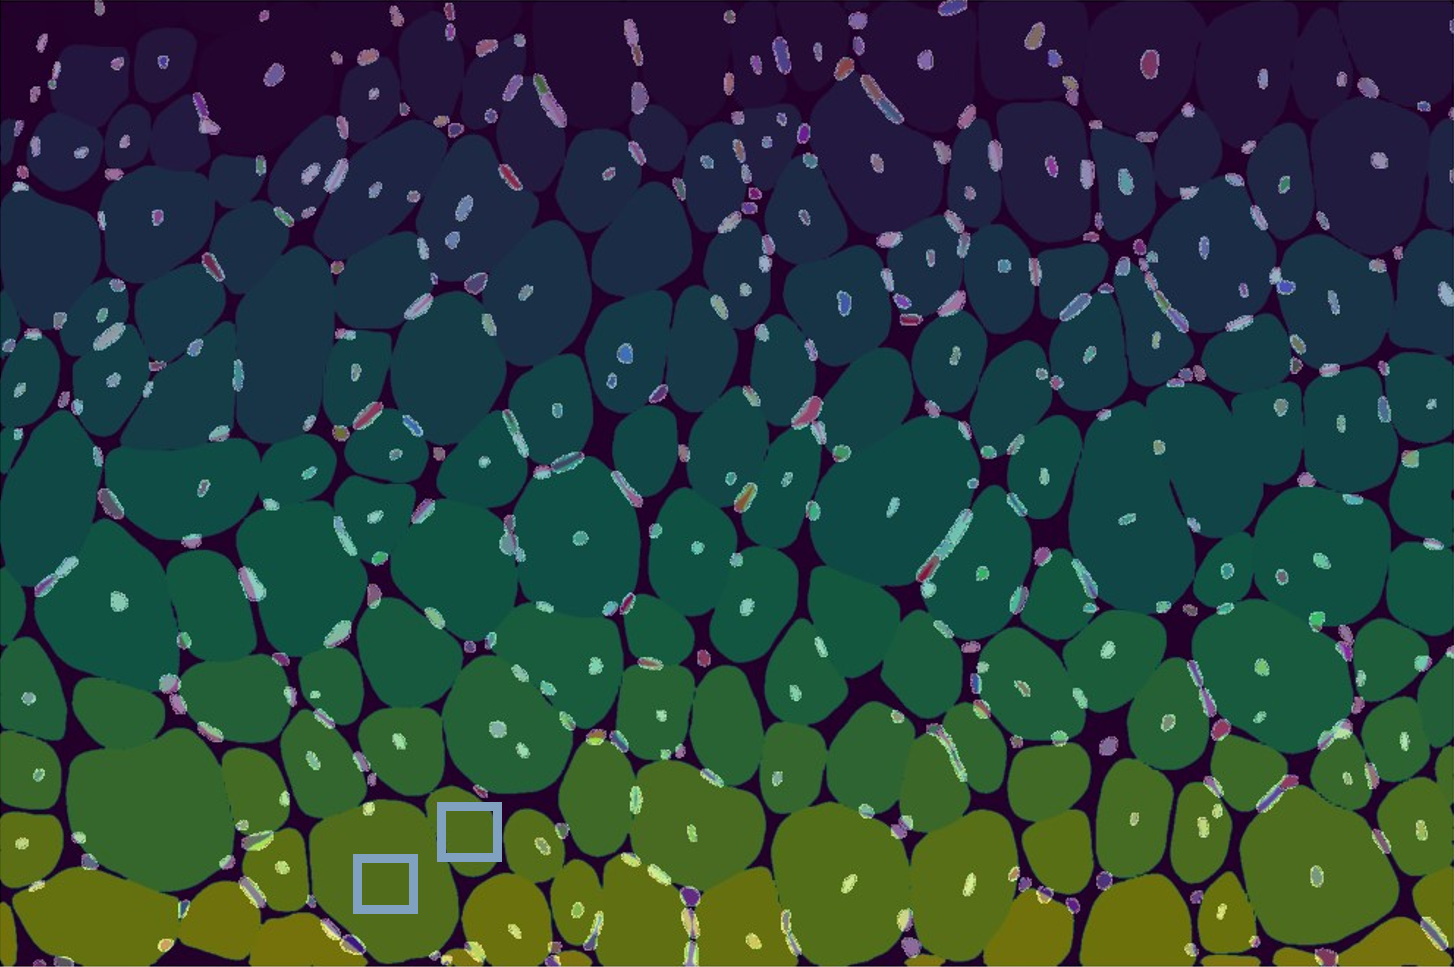
\includegraphics[width=0.8\textwidth]{figures/he_seg.png}
 \caption[Exemple de segmentation de biopsie par Cellpose et Stardist]{\textbf{Exemple de segmentation des fibres musculaires et des noyaux cellulaires par Cellpose et Stardist}. Chaque fibre musculaire segmentée est représentée en dégradé de jaune à bleu. Les noyaux détectés par Stardist sont représentés en surbrillance blanche. Les carrés bleus indiquent deux noyaux présents dans la coupe histologique originale, mais non détectés par Stardist.}
 \label{fig:he_seg}
\end{figure}

Après avoir obtenu la position de chaque fibre et noyau, nous évaluons la position de chaque noyau, fibre par fibre. Cette évaluation repose sur le calcul de ce que l'on appelle un score d'excentricité. Ce score est calculé selon la formule suivante:

\(\text{Score d'excentricité} = \frac{\text{Dist. centre fibre et noyau}}{\text{Dist. centre fibre et membrane}}\)

Dans cette formule, la notation "Dist. centre fibre et noyau" représente la distance en pixels entre le centroïde de la fibre musculaire et centroïde du noyau considéré. Et la notation "Dist. centre fibre et membrane" représente la distance entre le centroïde de la fibre musculaire et la membrane cellulaire selon une droite passant par le noyau d'intérêt. La figure \ref{fig:he_single_nuc} présente la classification des noyaux d'une fibre musculaire unique. Quatre noyaux ont été détectés dans cette fibre dont trois ont un score d'excentricité supérieur à 0,9 et un inférieur à 0,1. En fixant un seuil de façon empirique à 0,75, on considère alors que cette fibre musculaire possède un noyau internalisé.
\begin{figure}[!ht]
 \centering
 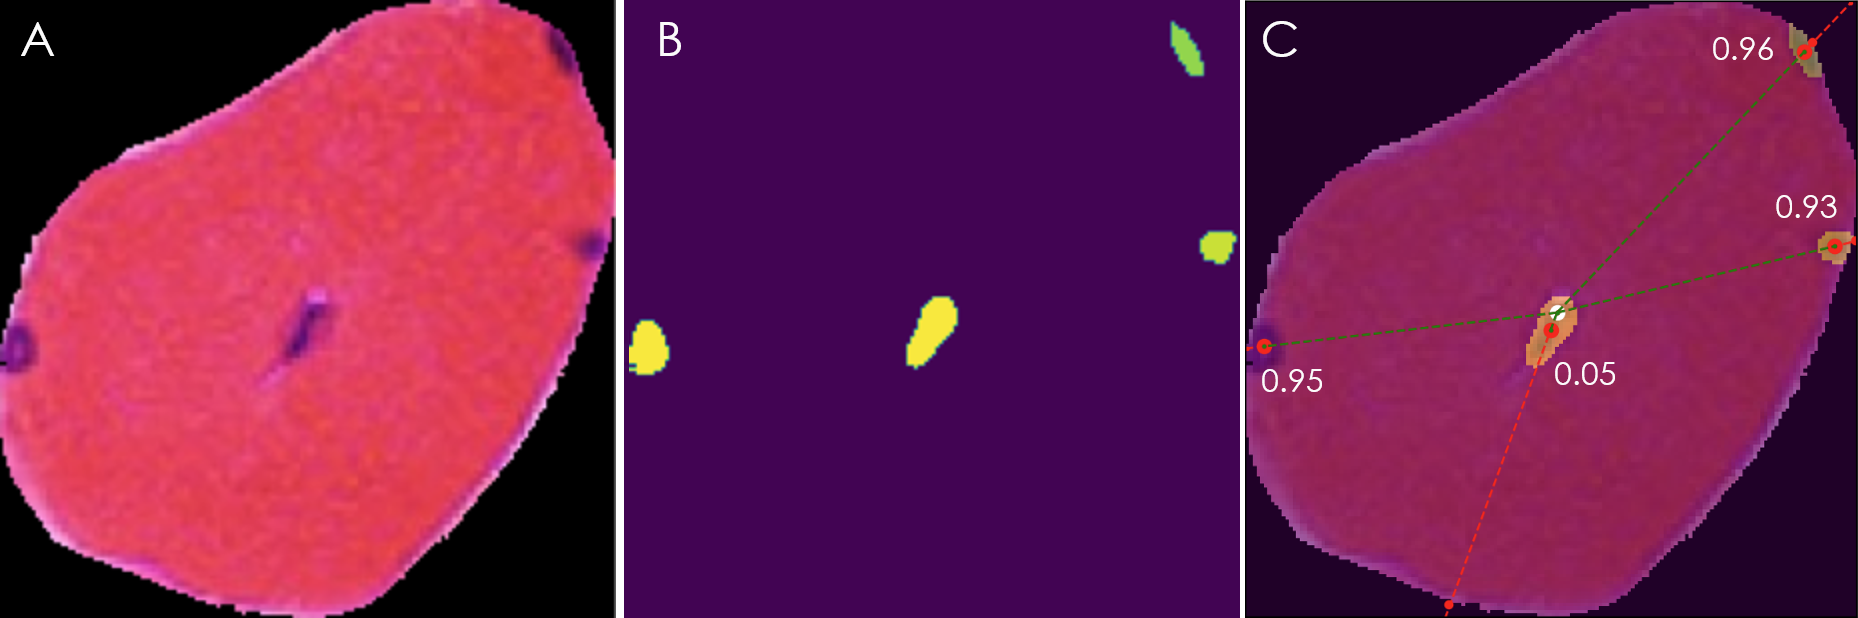
\includegraphics[width=1\textwidth]{figures/he_single_nuc.png}
 \caption[Exemple de classification de la position des noyaux]{\textbf{Exemple de classification de la position des noyaux cellulaires d'une fibre musculaire.} \textbf{(A)} La fibre musculaire seule \textbf{(B)} masque de segmentation des 4 noyaux pour cette fibre \textbf{(C)} schéma de la classification des noyaux avec le score d'excentricité de chaque noyau représentant le ratio de distance: centre de la fibre - noyau versus centre de la fibre - membrane cellulaire.}
 \label{fig:he_single_nuc}
\end{figure}
En comparant l'ensemble des noyaux de chaque fibre au seuil de 0.75, on peut alors quantifier le nombre de fibres musculaires ayant au moins un ou plusieurs noyaux internalisés. Par exemple, pour l'image présentée en figure \ref{fig:he_example}, la figure \ref{fig:he_paint} présente les résultats de cette classification. Sur cette coupe histologique, on obtient un total de 74 fibres (soit 42\% des fibres) avec au moins un noyau internalisé. Cependant, on observe que pour certaines fibres cette détection n'est pas correcte. Par exemple, représenté par un carré bleu et une flèche bleue, on observe trois fibres avec un noyau centralisé, mais considéré comme des fibres avec uniquement des noyaux périphériques. Cela s'explique, car de par leur faible coloration, les noyaux centraux n'ont pas été détectés correctement.
\begin{figure}[!ht]
 \centering
 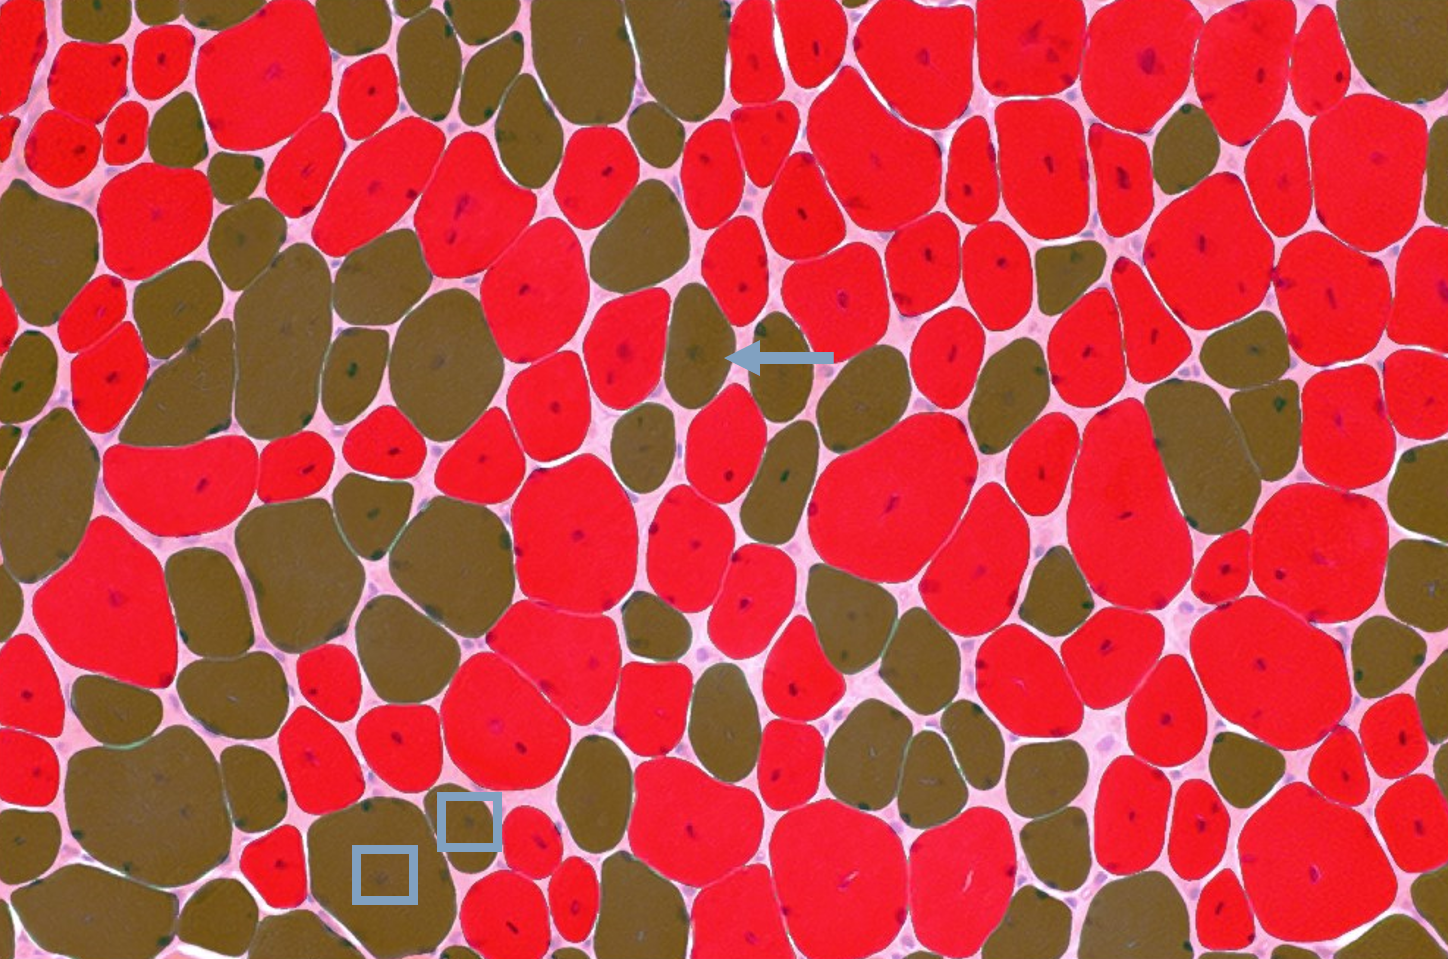
\includegraphics[width=0.8\textwidth]{figures/he_paint.png}
 \caption[Exemple de classification de biopsie musculaire à la coloration HE]{\textbf{Exemple de classification de biopsie musculaire à la coloration HE. }Colorées en vert les fibres sans noyau internalisé, et en rouge les fibres avec au moins un noyau internalisé (score d'excentricité inférieur à 0.75). Les carrés bleus et la flèche bleue indiquent des fibres dont la classification est fausse (considérées comme n'ayant pas de noyau centralisé).}
 \label{fig:he_paint}
\end{figure}

\subsection{Exemple d'application: quantification de la régénération musculaire }
La présence de noyaux centralisés dans les fibres musculaires est un marqueur pathologique dans les biopsies de \gls{mc}. Cependant, cette centralisation peut aussi être synonyme de régénération musculaire chez les individus sains. Ainsi, la quantification du nombre de noyaux centralisés est donc aussi un moyen de quantifier la régénération musculaire dans une coupe histologique. Dans le cadre d'une collaboration avec l'\gls{igbmc} et plus spécifiquement, avec l'équipe Biologie moléculaire et cellulaire des cancers du sein du Dr. Tomasetto, nous avons utilisé \gls{myoquant} pour évaluer la quantité de régénération musculaire chez des souris traitées avec une drogue induisant le processus régénératif. Ces images d'histologie sont des images à fluorescence (et non à la coloration \gls{he}) avec un fluorochrome pour la membrane cellulaire et un fluorochrome pour les noyaux cellulaires. L'algorithme de \gls{myoquant} est directement compatible avec les images à fluorescence et fonctionne de la même façon que pour les images à coloration\gls{he}
\begin{figure}[!ht]
 \centering
 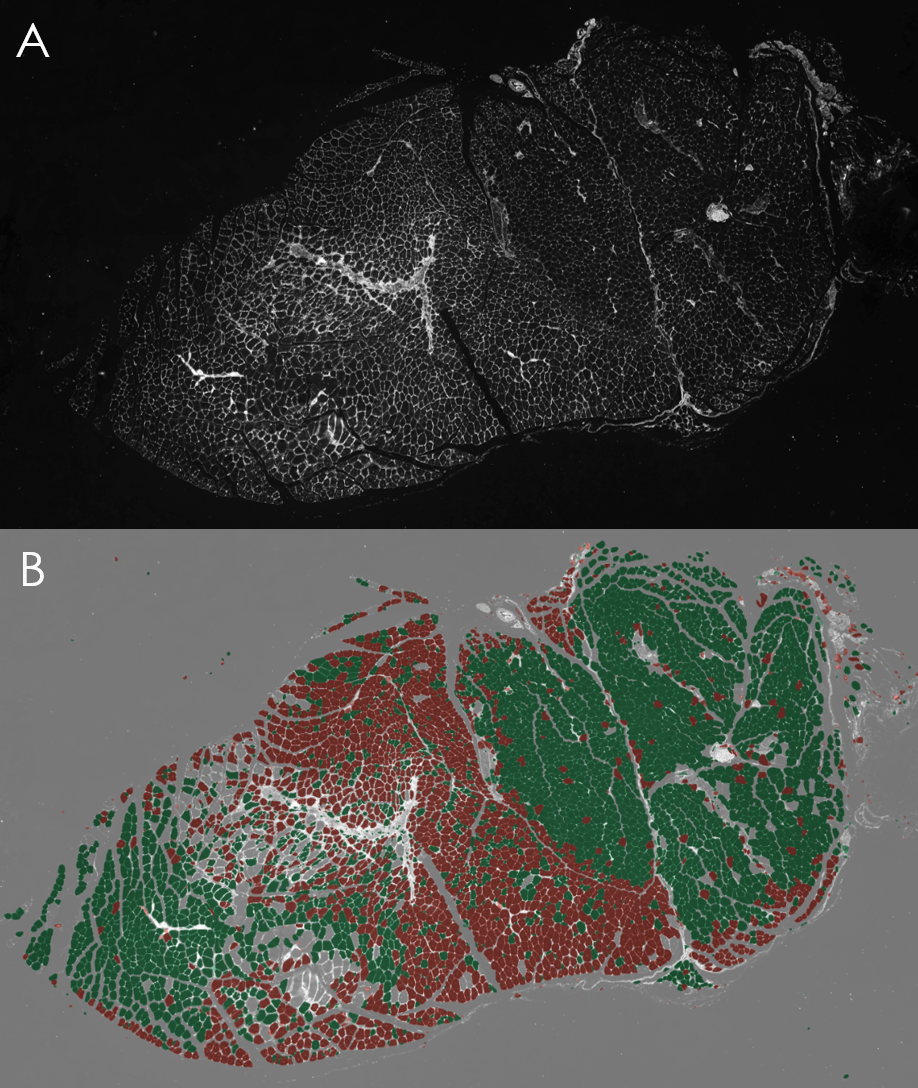
\includegraphics[width=0.8\textwidth]{figures/fluo_nuc.png}
 \caption[Exemple de classification de biopsie musculaire pour la régénération musculaire]{\textbf{Exemple de classification de biopsie musculaire pour la régénération musculaire.} \textbf{(A)} Image complète de la biopsie musculaire en microscopie à fluorescence.\textbf{ (B)} Classification des fibres de la biopsie musculaire par l'algorithme d'analyse des centralisations nucléaires. Colorées en vert les fibres sans noyau internalisé (fibres normales), en rouge les fibres avec au moins un noyau internalisé (en régénération)}
 \label{fig:fluo_paint}
\end{figure}

La figure \ref{fig:fluo_paint} présente un exemple de coupe complète de biopsie musculaire de souris avec le masque de quantification associé généré par \gls{myoquant}. Sur cette image, il y a 6078 fibres musculaires détectées, dont 2285 (environ 37\%) sont en régénération. Le tableau \ref{tab:myoquant_fluo_time} présente le temps de calcul nécessaire pour chaque étape de la quantification pour la coupe \ref{fig:fluo_paint} et le tableau \ref{tab:myoquant_fluo_results} présente les résultats de cette quantification. Une heure de temps de calcul a été nécessaire pour traiter une coupe complète sur une machine classique sans \gls{gpu}. La majorité de ce temps de calcul a été utilisée par Cellpose pour segmenter les fibres musculaires. Cependant, cette vitesse peut être largement améliorée d'un facteur 5 par l'utilisation de matériel spécifique aux calculs \gls{ia} (\gls{gpu}), passant d’environ 1 heure pour Cellpose à moins de 11 minutes. Le temps de calcul de Stardist et de classification des noyaux est négligeable (moins de 1m30). Ainsi, pour une image contenant 6078 fibres et 23 628 noyaux, cela représente environ 1.6 fibre traitée par seconde. Cette quantification a mis en évidence que 37\% des fibres présentaient un noyau internalisé et donc sont en régénération.
\begin{table}[!ht]
\centering
\caption[Temps de calcul pour l'analyse des noyaux d'une coupe complète à fluorescence]{\textbf{Temps de calcul pour l'analyse des noyaux d'une coupe complète à fluorescence} (6078 fibres, 12000 x 9600 pixels). La classification complète d'une coupe dure environ 1h sur CPU contre 12 minutes sur GPU soit une accélération d'un facteur 5.}
\label{tab:myoquant_fluo_time}
\begin{tabularx}{\textwidth}{|l|c|c|X|}
\hline
\textbf{Étape} & \textbf{Temps sur GPU} & \textbf{Temps sur CPU (s)} & \textbf{Fibres par seconde (sur CPU)} \\
\hline
Cellpose & 652 & 3 782 & 1.6 \\
\hline
StarDist & \textit{mémoire insuffisante} & 21 & 29 \\
\hline
Classification des noyaux & 68 & 68 & 89 \\
\hline
\textbf{Total} & \textbf{>720} & \textbf{3 871} & \textbf{1.57} \\
\hline
\end{tabularx}
\end{table}

\begin{table}[!ht]
\centering
\caption[Résultats de la quantification des noyaux d'une coupe complète à fluorescence]{\textbf{Résultats de la quantification des noyaux d'une coupe complète à fluorescence} (6078 fibres, 12000 x 9600 pixels). Au total, 37\% des 6078 fibres ont été détectées comme ayant au moins un noyau centralisé (donc en régénération dans ce cas de figure).}
\label{tab:myoquant_fluo_results}
\begin{tabular}{|l|c|c|}
\hline
\textbf{Type} & \textbf{Valeur} & \textbf{Proportion (\%)} \\
\hline
N° Fibres & 6 078 & 100 \\
\hline
N° Fibres avec 1+ noyau internalisé & 2 264 & 37 \\
\hline
\hline
N° Noyaux & 23 628 & 100 \\
\hline
N° Noyaux internalisés & 3 933 & 16 \\
\hline
N° Noyaux périphériques & 17 918 & 76 \\
\hline
N° Noyaux non classés (hors fibres) & 1 777 & 8 \\
\hline
\end{tabular}
\end{table}
Le tableau \ref{fig:fluo_compil} présente l'ensemble des quantifications opérées dans les différentes conditions de traitement et de génotype (au total 35 \gls{wsi} analysées). On observe qu'après traitement avec la \textit{Cardiotoxin}, une drogue induisant la régénération musculaire, une proportion significativement supérieure de fibres ayant un noyau internalisé par rapport aux coupes contrôle. Ces résultats confirment que \gls{myoquant} est bien capable d'évaluer de façon robuste la présence de noyaux internalisés, un marqueur de la régénération musculaire.

\begin{figure}[!ht]
 \centering
 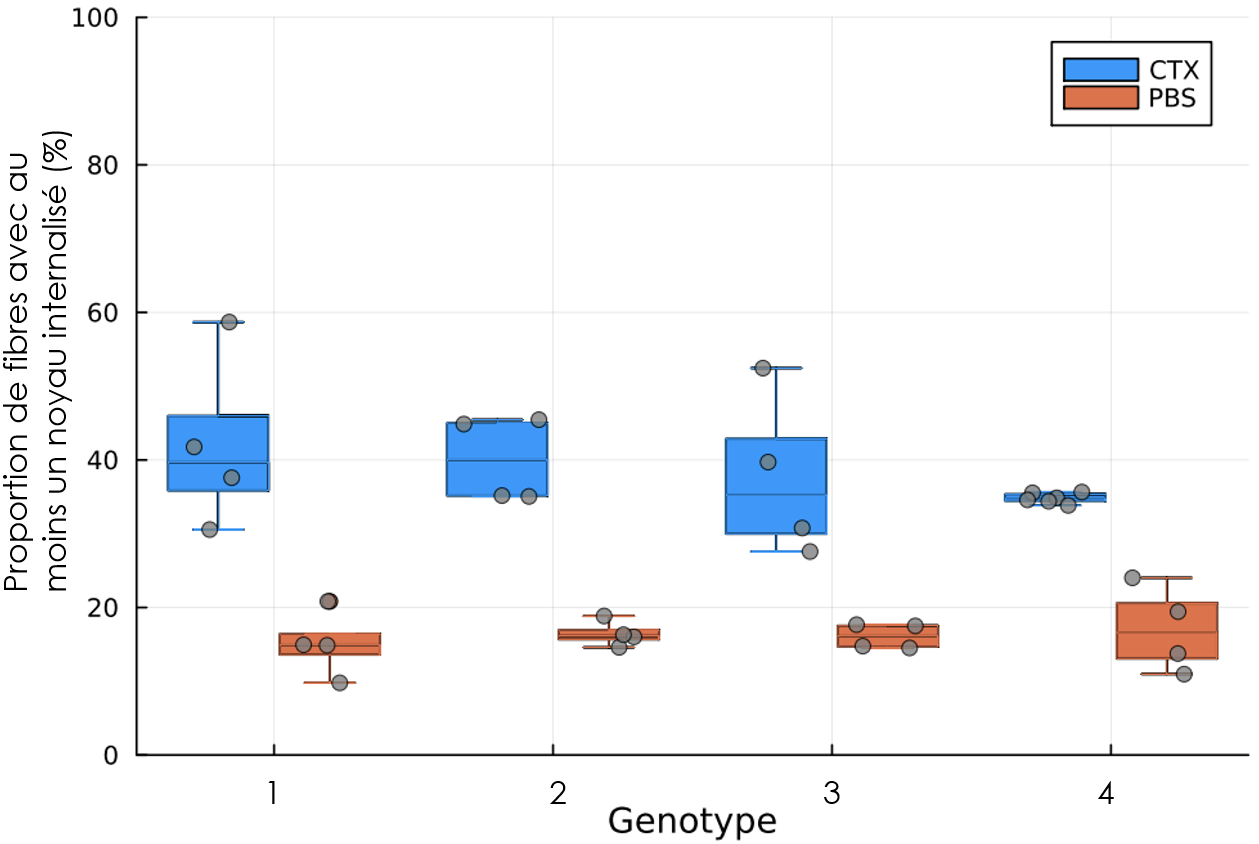
\includegraphics[width=0.8\textwidth]{figures/fluo_compil.png}
 \caption[Résultat de la quantification de la régénération musculaire]{\textbf{Résultat de la quantification de la régénération musculaire chez des souris pour 4 génotypes différents }. En bleu sont représentées les souris traitées (bleu) avec une drogue induisant la régénération musculaire (\textit{Cardiotoxin}, CTX). En orange sont représentées les souris de contrôle (solution saline de tampon, PBS).}
 \label{fig:fluo_compil}
\end{figure}

\section{Ratio de fibre de type 1 et 2: classification basée sur l'intensité de coloration}

Dans un second temps, nous nous sommes intéressés à l'analyse du ratio des différents types de fibres musculaires dans les biopsies. Dans certaines \gls{mc}, l'équilibre entre fibres de type 1 (fibre à contraction lente et endurante) et type 2 (fibre à contraction rapide) peut être modifié avec une prédominance des fibres de type 1. Ces deux types de fibres musculaires ont une intensité de coloration différente à la coloration ATPase. À un pH 4.3, les fibres de type 1 sont sombres et les fibres de type 2 sont pâles, et inversement au pH 9.4. La figure \ref{fig:atp_example} représente une biopsie musculaire colorée à l'ATPase pH 9.4. On observe assez bien la présence des deux populations de fibres à intensité de coloration distincte et nous avons mis à profit ces différences d'intensité pour développer une méthode de comptage automatique du nombre de fibres de chaque type.
\begin{figure}[!ht]
 \centering
 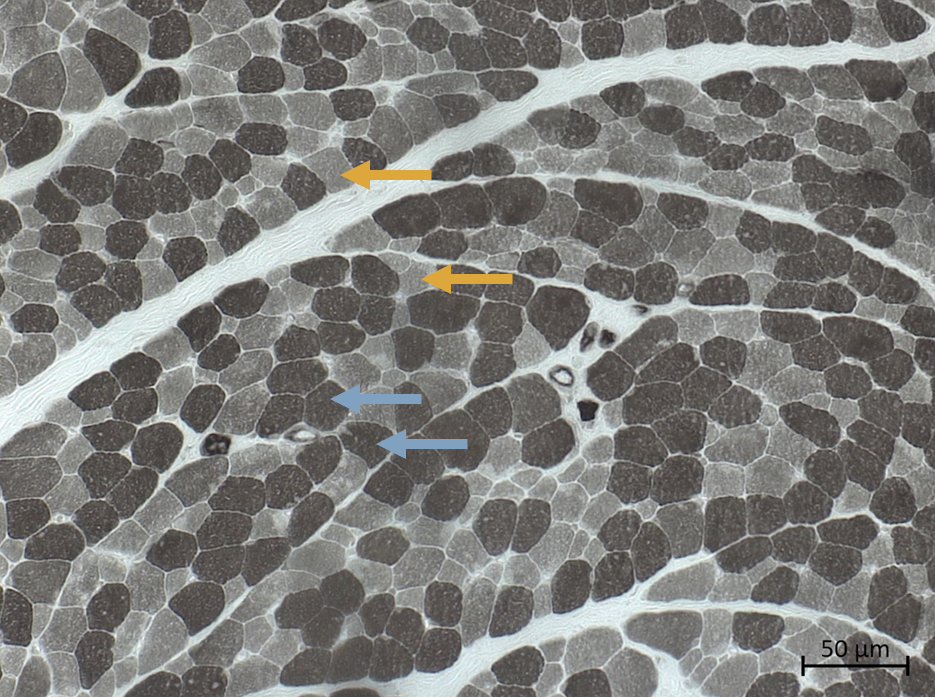
\includegraphics[width=0.8\textwidth]{figures/atp_example.png}
 \caption[Exemple de biopsie musculaire à la coloration ATPase pH 9.4]{\textbf{Exemple de biopsie musculaire à la coloration ATPase pH 9.4}. Cette coloration permet de différencier les fibres de type 1 (flèches jaunes) aux fibres de type 2 (flèches bleues).}
 \label{fig:atp_example}
\end{figure}
\subsection{Algorithme de quantification}
Pour réaliser cette quantification, la première étape consiste à segmenter, c'est-à-dire obtenir la position de toutes les fibres musculaires. Comme précédemment, nous avons utilisé Cellpose afin de segmenter les fibres musculaires. Ensuite, pour chaque fibre, nous avons extrait l'intensité moyenne de la fibre et avons réalisé un histogramme. La figure \ref{fig:atp_density} présente l'histogramme issu de l'analyse de l'image d'exemple pour la coloration ATPase pH 9.4 (\ref{fig:atp_example}). Le but de la procédure est de déterminer automatiquement les pics présents dans l'histogramme et de trouver les minimums locaux entre les pics pour fixer un ou plusieurs seuils d'intensité. Pour cela, à partir des valeurs de cet histogramme, une courbe de densité est créée (par méthode de \gls{kde}). Puis à partir de cette courbe de densité, une méthode de mélange gaussien est utilisée pour déterminer la position des pics dans la courbe de densité. Finalement, le seuil est déterminé automatiquement par notre méthode en trouvant le minimum local de la courbe de densité entre les deux pics obtenus par mélange gaussien.
\begin{figure}[!ht]
 \centering
 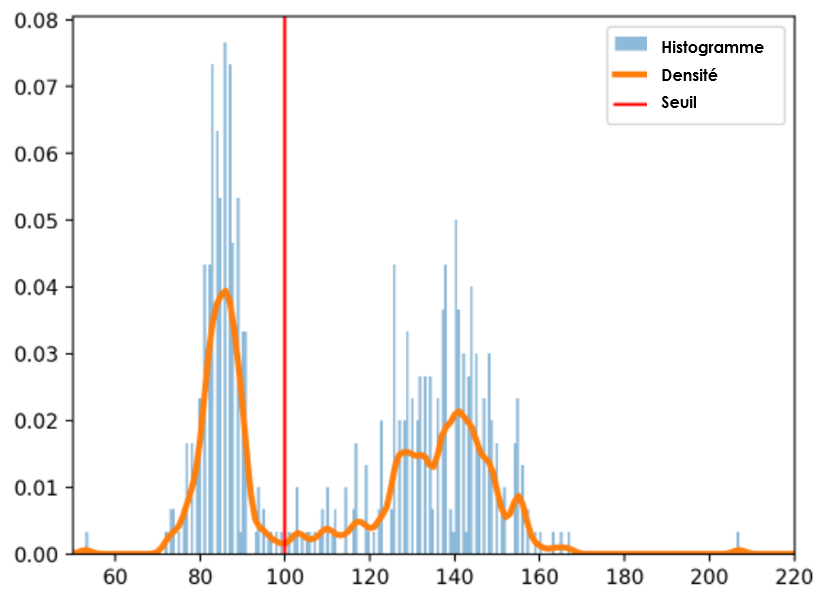
\includegraphics[width=0.8\textwidth]{figures/density_plot.png}
 \caption[Exemple d'histogramme et courbe de densité biopsie ATPase]{\textbf{Exemple d'histogramme et courbe de densité biopsie ATPase}. L'histogramme en bleu représente les valeurs moyennes d'intensité de chaque cellule détectée. La courbe en orange est la courbe de densité représentant la distribution des intensités de coloration des cellules. La barre verticale rouge représente le seuil d'intensité défini automatiquement par l'algorithme pour une classification des fibres en deux classes.}
 \label{fig:atp_density}
\end{figure}

À partir de ce seuil, il est possible de classer les fibres musculaires en deux catégories: celles avec une intensité moyenne inférieure au seuil et celles avec une intensité moyenne supérieure. La figure \ref{fig:apt_paint} présente les résultats de la quantification automatique des fibres de l'image présentée en exemple précédemment. Sur cette image, on a pu quantifier au total la présence de 496 fibres, dont 269 (54\%) fibres de type 1 et 227 (46\%) fibres de type 2. 
\begin{figure}[!ht]
 \centering
 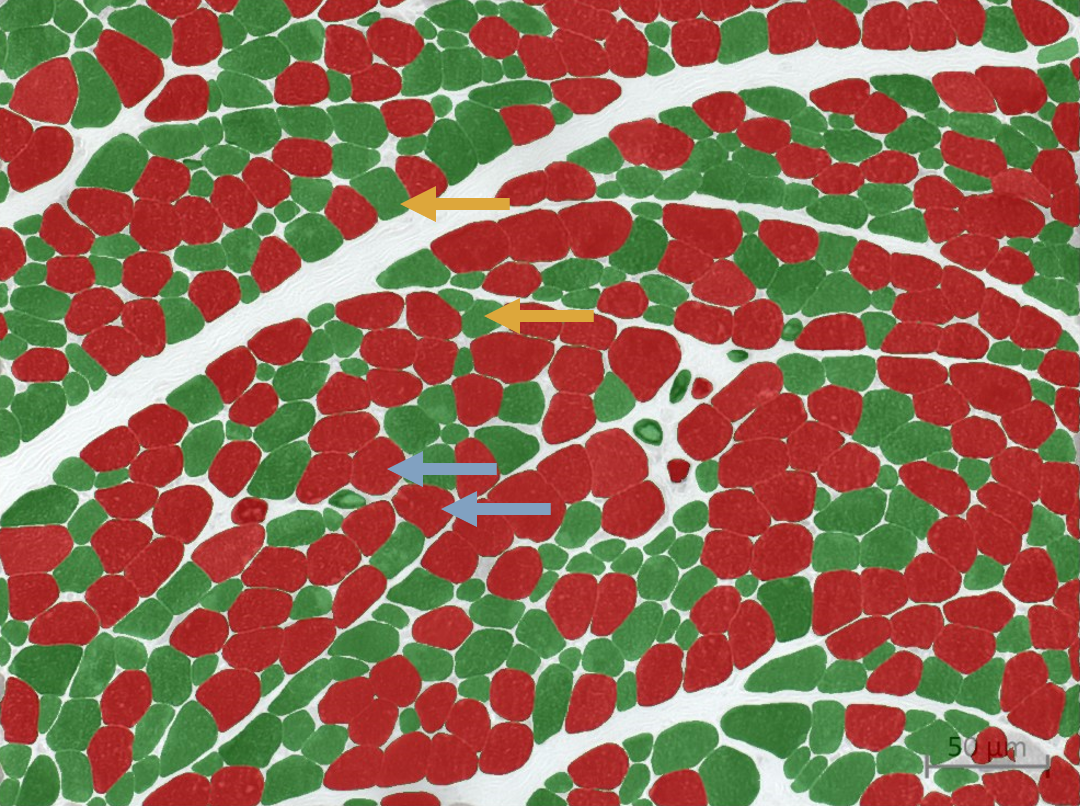
\includegraphics[width=0.8\textwidth]{figures/atp_paint.png}
 \caption[Exemple de classification de biopsie musculaire à la coloration ATPase pH 9.4]{\textbf{Exemple de classification de biopsie musculaire à la coloration ATPase pH 9.4.} Les fibres ayant une intensité inférieure au seuil (type 2, flèches bleues) sont colorées en rouge. Les fibres ayant une intensité supérieure au seuil (type 1, flèches jaunes) sont colorées en vert.}
 \label{fig:apt_paint}
\end{figure}

\subsection{Exemple d'application: classification d'une coupe complète avec trois types de fibres}
La coloration ATPase peut révéler plus de deux types de fibres musculaires. En effet, les fibres de type 2 ont plusieurs sous-types visualisables dans certaines conditions de coloration. Dans cet exemple, nous avons utilisé la méthode de classification développée pour détecter trois types de fibres. La méthode que nous avons développée est capable d'établir autant de seuils automatiquement que spécifiés par l'utilisateur (et donc de classes). La figure \ref{fig:atp_paint_wsi} présente les résultats de classification d'une \gls{wsi} de biopsie musculaire colorée à l'ATP pH 4.6. Sur cette coupe, on observe trois populations de fibres: des fibres pâles (fibres de type 2A, flèche noire), des fibres intermédiaires (fibres de type 2B, flèche blanche) et de petites fibres très sombres localisées en haut de la coupe (fibres de type 1, flèche verte). La méthode de quantification a alors pu définir deux seuils pour séparer ces trois classes. 
\begin{figure}[!ht]
 \centering
 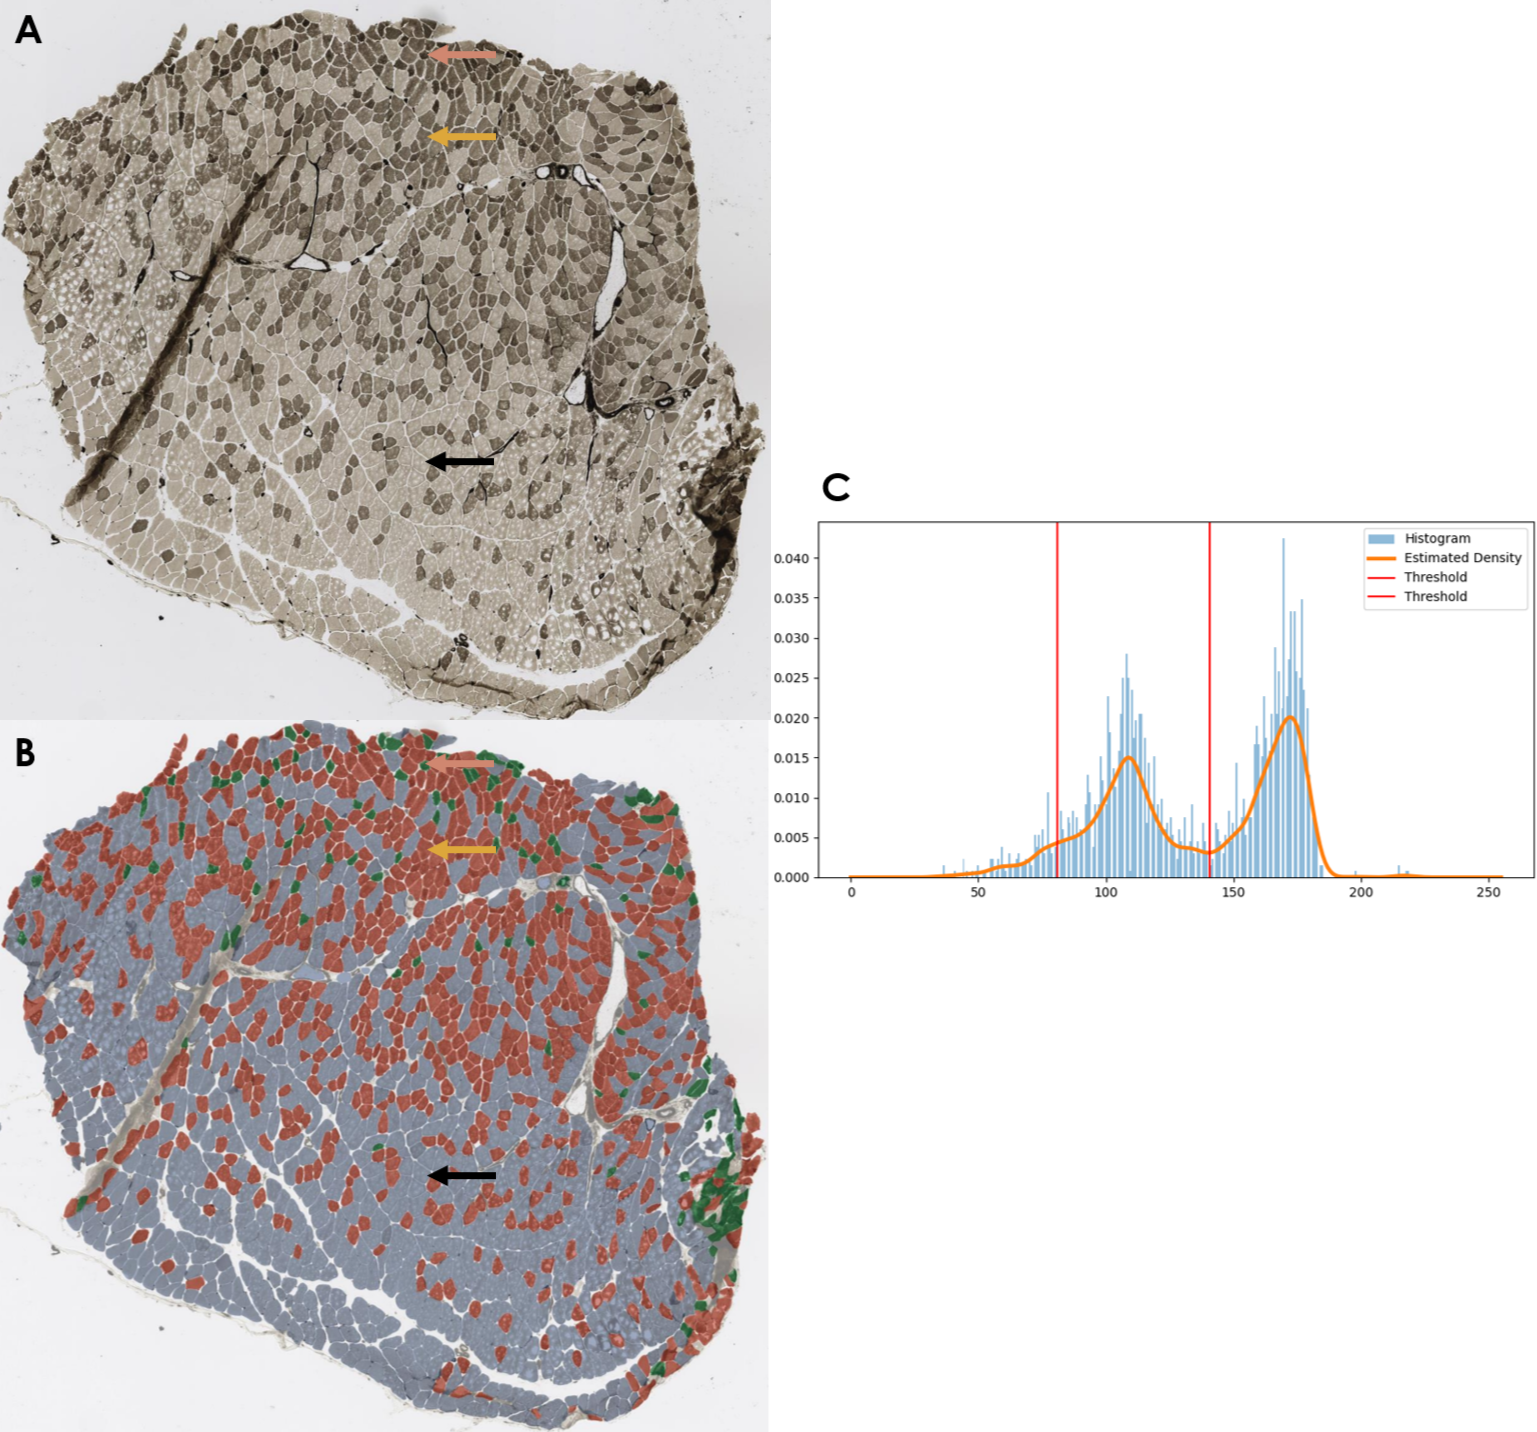
\includegraphics[width=1\textwidth]{figures/atp_wsi.png}
 \caption[Exemple de classification de biopsie musculaire colorée à l'ATPase]{\textbf{Exemple de classification de biopsie musculaire colorée à l'ATPase pH 4.6 en 3 classes}. \textbf{(A)} Image brute de biopsie musculaire ATPase pH 4.6. Pointées par une flèche noire les fibres 2A, blanche les fibres 2B et verte les fibres type 1 \textbf{(B)} Image de biopsie dont les fibres ont été colorées en fonction de leur classification: en bleu les fibres de type 2A, en rouge les fibres de type 2B et en vert les fibres de type 1. \textbf{(C)} Histogramme et courbe de densité des fibres de la biopsie complète.}
 \label{fig:atp_paint_wsi}
\end{figure}

Les résultats de cette classification sont référencés dans le tableau \ref{tab:atp_wsi_resultstable}, le temps de calcul et la vitesse de classification sont disponibles dans le tableau \ref{tab:atp_wsi_timetable}. Au total, 1840 fibres ont été classifiées en 131 secondes (soit 14 fibres par seconde). Il y a une majorité de fibres de type 2A (894, 49\%), de fibres de type de 2B (829, 45\%) et une faible proportion de petites fibres de type 1 (117, 6\%). Les résultats de cette quantification sont visuellement satisfaisants, bien qu'une partie de la biopsie en bas à droite, est repliée sur elle-même et donc apparait avec une intensité de coloration forte. Cette zone a donc été considérée à tort comme des fibres de type 1. 

Ces résultats montrent qu'il est nécessaire d'améliorer la robustesse de la méthode de quantification pour prendre en compte la variabilité des échantillons biologiques. En plus des repliements qui influent sur l'intensité de coloration, il peut aussi y avoir des artéfacts de congélations (zone sous forme de bulles blanches dans les fibres, visibles sur la partie gauche de la coupe) qui eux aussi faussent le calcul de l'intensité moyenne des fibres. De fait, il peut être nécessaire d'avoir des méthodes de filtrage en amont de la classification pour ne quantifier que les fibres de bonne qualité, ou d'éliminer au préalable les zones très hétérogènes.

\begin{table}[!ht]
\centering
\caption[Temps de calcul pour l'analyse des types de fibres d'une coupe complète ATPase]{\textbf{Temps de calcul pour l'analyse des types de fibres d'une coupe complète à la coloration ATPase pH 4.6} (1840 fibres, 6000 x 5600 pixels). La classification complète d'une coupe composée de 1840 fibres sur GPU dure au total 2 minutes et 11 secondes.}
\label{tab:atp_wsi_timetable}
\begin{tabular}{|l|c|c|}
\hline
\textbf{Étape} & \textbf{Temps sur GPU} & \textbf{Fibre par seconde (sur GPU)} \\
\hline
Cellpose & 113 & 16 \\
\hline
Classification des fibres & 18 & 102 \\
\hline
\textbf{Total} & \textbf{131} & \textbf{14} \\
\hline
\end{tabular}
\end{table}
\begin{table}[!ht]
\centering
\caption[Résultats de quantification des types de fibre d'une coupe complète ATPase]{\textbf{Résultats de quantification des types de fibre d'une coupe complète à la coloration ATPase pH 4.6} (1840 fibres, 6000 x 5600 pixels). Sur cette coupe complète, on obtient un ratio presque égal de fibre 2A et 2B (49\% et 45\% respectivement) ainsi qu'une très petite proportion de fibres de type 1 (petites fibres fortement colorées, 6\%).}
\label{tab:atp_wsi_resultstable}
\begin{tabular}{|l|c|c|}
\hline
\textbf{Type} & \textbf{Valeur} & \textbf{Proportion (\%)} \\
\hline
Fibre type 2A & 894 & 49 \\
\hline
Fibre type 2B & 829 & 45 \\
\hline
Fibre type 1 & 117 & 6 \\
\hline
\end{tabular}
\end{table}


\section{Répartition des mitochondries: classification par IA}
Enfin, nous nous sommes intéressés à l'analyse de la répartition des mitochondries dans les fibres musculaires. Cette répartition peut être anormale dans certaines \gls{mc}. Cette répartition se visualise grâce à la coloration \gls{sdh}, révélant l'activité oxydative des fibres musculaires et donc la position des mitochondries. La figure \ref{fig:sdh_example} présente un exemple de biopsie de muscle d'une souris modèle de myopathie congénitale à la coloration \gls{sdh}. On observe deux types de fibres, des fibres "normales" (indiqué par des flèches noires) ayant une répartition homogène en coloration et des fibres "anormales" ayant une agglutination de coloration au centre de la fibre (indiqués par des flèches rouges), représentant des agrégats mitochondriaux pathologiques. Dans ce cadre, nous avons développé une méthode capable de détecter et de compter les fibres ayant une répartition mitochondriale anormale, en développant notre propre modèle d'\gls{ia}.

\begin{figure}[!ht]
 \centering
 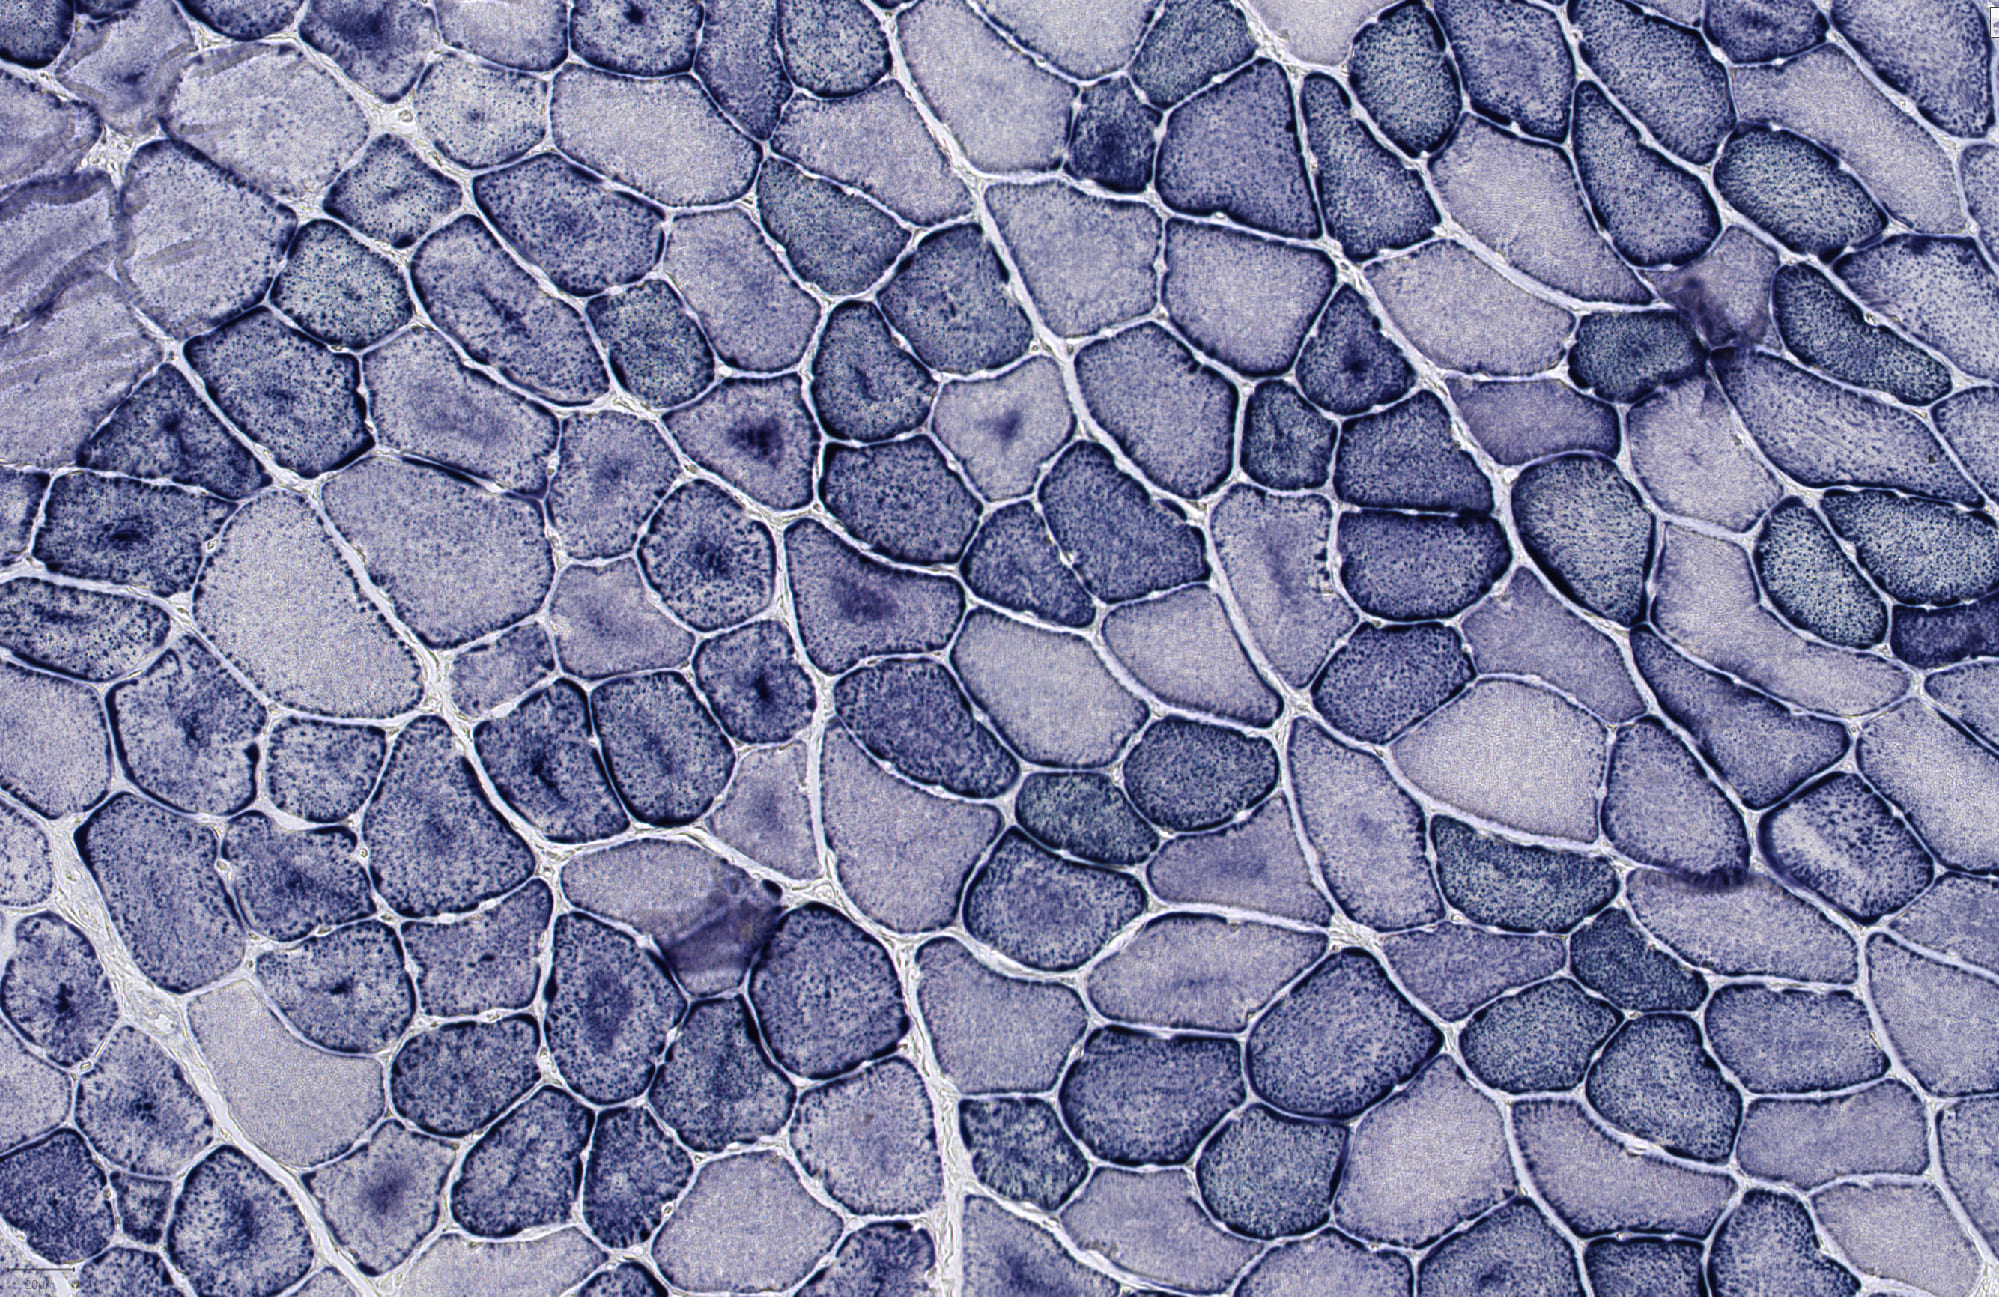
\includegraphics[width=0.8\textwidth]{figures/sdh_example.png}
 \caption[Exemple de biopsie musculaire à la coloration SDH]{\textbf{Exemple de biopsie de muscle de souris modèle de CNM à la coloration SDH}. Les flèches noires pointent des fibres ayant une répartition de coloration normale. Les flèches rouges pointent des fibres ayant une coloration anormale avec une tache sombre centrale. Ces fibres ont une répartition mitochondriale pathologique.}
 \label{fig:sdh_example}
\end{figure}
\subsection{Jeu de données d'image de muscle de souris et annotations}
Pour constituer le jeu de données nécessaire à l'entrainement de cette \gls{ia} nous avons utilisés 18 \gls{wsi} de biopsies musculaires de souris, dont une souris saine (\textit{wild-type}) et 17 \gls{wsi} de souris modèles de \gls{cnm} (10 \textit{Bin1-KO} et 7 \textit{Dnm2S619L}). Ces 18 \gls{wsi} représentent un total de 16 787 fibres musculaires (tableau \ref{tab:sdh_fiber_count}). Chacune de ces fibres musculaires a été isolée et extraite de la coupe grâce à Cellpose puis a été annotée à la main en 2 catégories: fibre saine ou anormale, par l'expert ayant généré les images (Quentin Giraud et Charlotte Gineste de l'équipe "Physiopathologie des maladies neuromusculaires" de l'\gls{igbmc}). Au total, les 12 730 fibres saines et 4 057 fibres annotées comme anormales ont été séparées équitablement en trois jeux de données: 72\% pour le jeu d'entrainement de l'\gls{ia}, 8\% pour le jeu de validation lors de l'entrainement, et 20\% pour le jeu de test des performances de l'\gls{ia}. Ce jeu de données a été mis à disposition de la communauté scientifique de façon \textit{open-source} sur la plateforme \textit{Hugging-Face} à l'adresse: \href{https://huggingface.co/datasets/corentinm7/MyoQuant-SDH-Data}{https://huggingface.co/datasets/corentinm7/MyoQuant-SDH-Data}.

\begin{table}[!ht]
\centering
\caption[Répartition des fibres pour le jeu d'entrainement du modèle SDH]{\textbf{Répartition des fibres pour le jeu d'entrainement du modèle SDH}. Malgré une répartition avec 1 coupe \textit{wild-type} et 17 coupes de souris modèle de \gls{mc}, on observe une majorité de fibre saine dans parmi les 16 787 fibres du jeu d'entrainement (76\%).}
\label{tab:sdh_fiber_count}
\begin{tabular}{|c|c|c|c|c|}
\hline
 & \textbf{Entraînement} (72\%) & \textbf{Validation} (8\%) & \textbf{Test} (20\%) & \textbf{Total} \\
\hline
\textbf{Saine} & 9 165 & 1 019 & 2 546 & 12 730 (76\%) \\
\hline
\textbf{Anormale} & 2 920 & 325 & 812 & 4 057 (24\%) \\
\hline
\hline
\textbf{Total} & 12 085 & 1 344 & 3 358 & 16 787 \\
\hline
\end{tabular}
\end{table}


\subsection{Architecture, entrainement et performance du modèle IA}
À partir de ce jeu de données, nous avons entrainé un modèle de \gls{cnn}. Nous avons sélectionné l'architecture réseau de neurones profonds \textit{Resnet50} pré-entrainée sur \textit{ImageNet}. L'architecture \textit{Resnet50} est une architecture de \gls{dnn} très utilisée pour la classification d'images et le pré-entrainement sur \textit{ImageNet} permet d'obtenir de meilleures performances et une convergence du modèle accélérée. Pour limiter le sur-apprentissage, nous avons appliqué des techniques d'augmentation de données lors de l'apprentissage par variation de luminosité, contraste, rotation aléatoire, zoom, translation et retournement. De plus, nous avons utilisé une méthode d'arrêt prématuré pour arrêter l'entrainement lorsque les performances sur le jeu de validation ne se sont pas améliorées lors des 10 dernières époques. Enfin, chaque fibre musculaire unique a été redimensionnée à une taille de 256x256 pixels, car le réseau de neurones impose une taille d'image constante.
\begin{figure}[!ht]
 \centering
 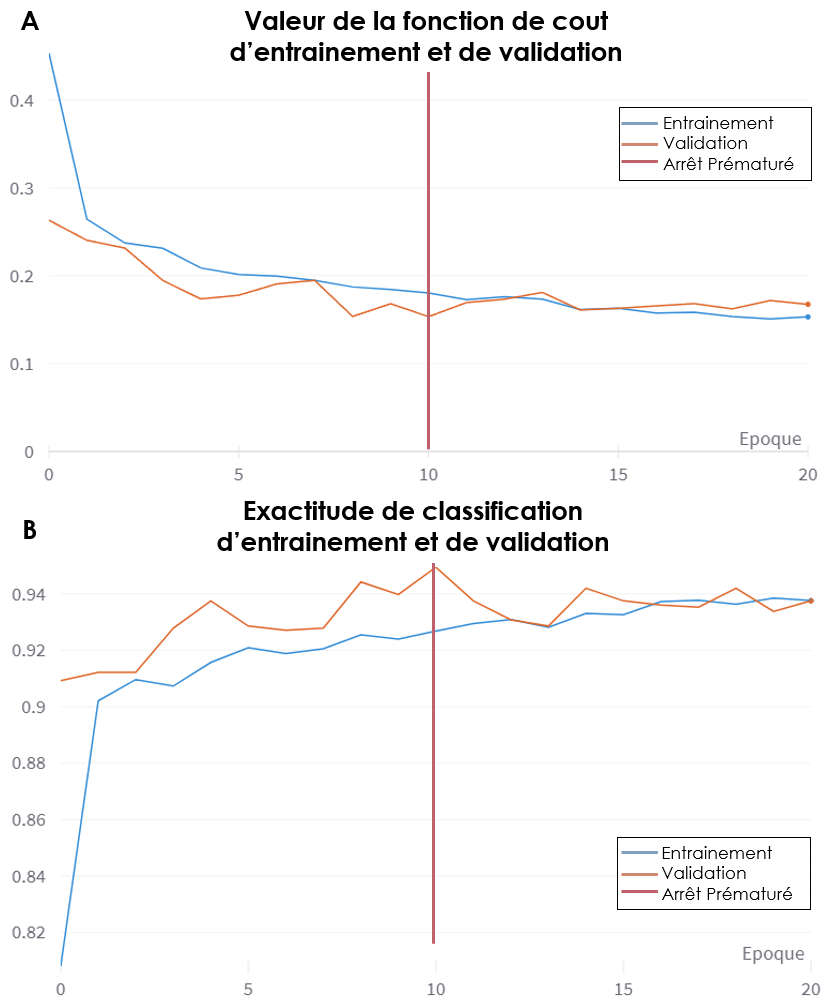
\includegraphics[width=1\textwidth]{figures/training_sdh.png}
 \caption[Courbe d'apprentissage du modèle SDH]{\textbf{Courbe d'apprentissage du modèle SDH.} \textbf{(A)} La courbe de la fonction de cout \textbf{(B)} La courbe d'exactitude de classification pour le jeu d'entrainement (bleu) et le jeu de validation (orange). La barre verticale rouge indique le modèle final sélectionné par le mécanisme d’arrêt prématuré.}
 \label{fig:sdh_train}
\end{figure}

La figure \ref{fig:sdh_train} présente les courbes d'apprentissage du modèle \gls{sdh}. Que ce soit en termes de mesure de la fonction de cout du modèle (\textit{loss function}) ou d'exactitude de classification, on observe qu'après 10 époques (12 minutes d'entrainement), les performances sont maximales pour le jeu de validation et ne s'améliorent plus sur les 10 époques suivantes. Ceci indique qu'après 10 époques, l'apprentissage donne lieu à un sur-apprentissage du jeu d'entrainement. C'est pourquoi grâce à l'arrêt prématuré, nous avons sélectionné le modèle dans l'état après 10 époques comme modèle optimal sans sur-apprentissage.

Après la phase d'apprentissage, pour mesurer les performances du modèle, nous avons utilisé le jeu de test composé de 3358 images non utilisées pour l'entrainement. En comparant les prédictions du modèle sur les images de test à leur annotation par les experts, nous avons obtenu une exactitude de classification de 93,2\% et une exactitude pondérée de 91.7\%. Autrement dit, le modèle est capable de reproduire l'annotation des deux experts avec une exactitude de 93,2\%.

L'ensemble des métriques mesurées lors de l'entrainement sont disponibles de façon open source à l'adresse: \href{https://wandb.ai/lambda-science/myoquant-sdh/reports/Model-Training---Vmlldzo0NDI4MDI4}{https://wandb.ai/lambda-science/myoquant-sdh/reports/Model-Training---Vmlldzo0NDI4MDI4}, le modèle ainsi que le code source utilisés pour réaliser cet entrainement de manière reproductible sont aussi disponibles sur la plateforme \textit{HuggingFace} à l'adresse: \href{https://huggingface.co/corentinm7/MyoQuant-SDH-Model}{https://huggingface.co/corentinm7/MyoQuant-SDH-Model}.

\subsection{Exemple d'application}
Grâce au modèle développé, il est maintenant possible de classer des fibres individuelles pour détecter les anomalies de répartition mitochondriale. Ainsi pour analyser une image complète, on utilise d'abord Cellpose pour segmenter et isoler chaque fibre musculaire de l'image, puis le modèle que nous avons développé pour prédire la classe de la fibre. Par exemple, pour l'image de biopsie présentée ci-dessus (\ref{fig:sdh_example}), le résultat de classification est présenté en figure \ref{fig:sdh_paint}. Au total, sur 162 fibres détectées, 86 (53\%) sont classées comme ayant une répartition mitochondriale anormale et 76 (46\%) ont une répartition normale. On observe que ce sont bien les fibres ayant une agglutination de coloration au centre de la fibre (agrégats de mitochondries, sur la gauche de la coupe) qui sont classées comme anormales, confirmant le bon fonctionnement du modèle.

\begin{figure}[!ht]
 \centering
 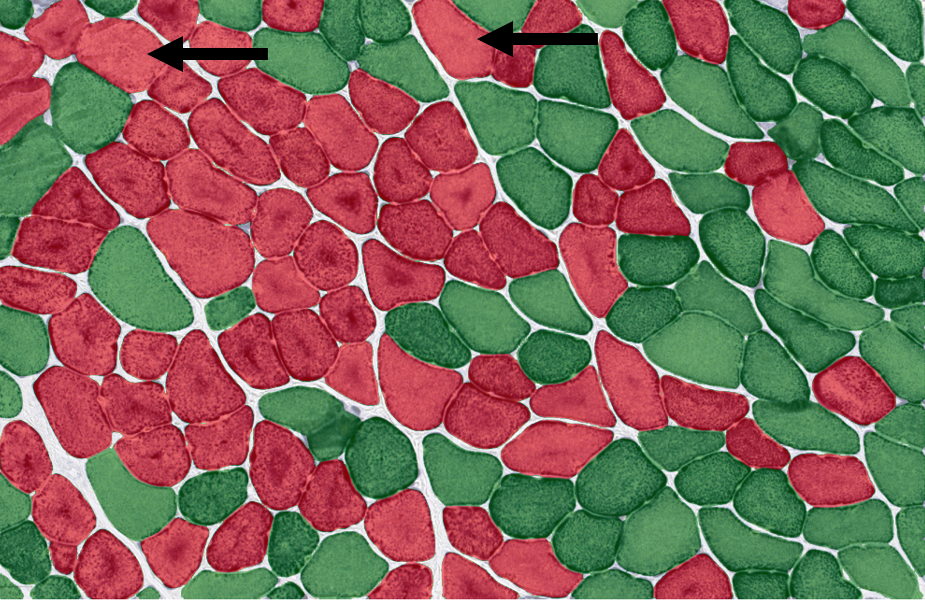
\includegraphics[width=0.8\textwidth]{figures/sdh_paint.png}
 \caption[Exemple de classification de biopsie musculaire de souris à la coloration SDH]{\textbf{Exemple de classification de biopsie musculaire de souris à la coloration SDH.} Colorées en rouge, les fibres ayant une répartition mitochondriale anormale, en vert, une répartition normale. Les fibres pointées par une flèche noire sont des fibres qui sont classées comme anormales, mais ayant une apparence saine (possible erreur de classification).}
 \label{fig:sdh_paint}
\end{figure}
\begin{figure}[!ht]
 \centering
 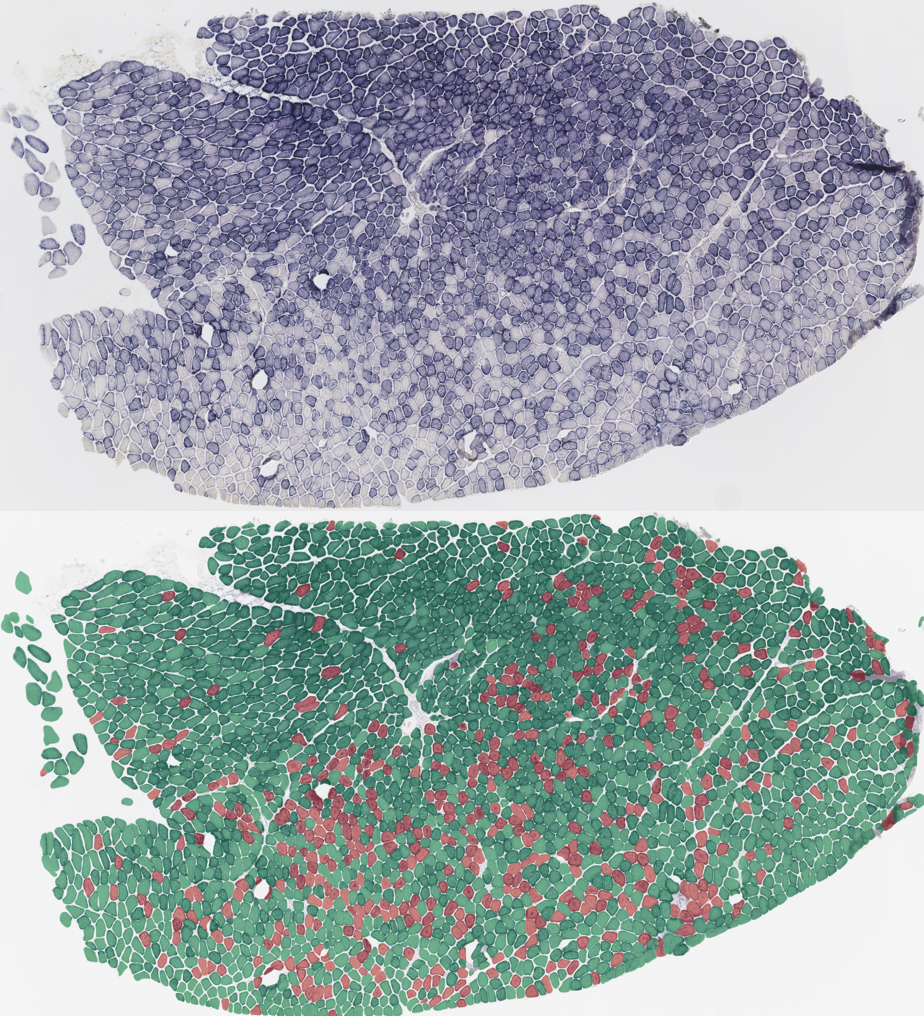
\includegraphics[width=0.8\textwidth]{figures/wsi_sdh.png}
 \caption[Exemple de classification de coupe complète biopsie musculaire de souris à la coloration SDH]{\textbf{Exemple de classification de coupe complète biopsie musculaire de souris à la coloration SDH.} \textbf{(A)} Biopsie musculaire complète de souris à la coloration SDH. \textbf{(B)} Biopsie musculaire complète dont les fibres ont été colorées en fonction de leur classification par le modèle \gls{ia}: en rouge les fibres ayant répartition mitochondriale anormale, en vert une répartition normale}
 \label{fig:sdh_wsi_paint}
\end{figure}

Il est aussi possible de classer des \gls{wsi} de biopsies de muscle complet colorées au \gls{sdh}. Par exemple, la figure \ref{fig:sdh_wsi_paint} présente les résultats de classification d'une coupe complète comptant 2 869 fibres musculaires. En termes de ressources de calcul, l'étape limitante reste le modèle Cellpose qui, pour cette image, requiert trop de mémoire pour fonctionner sur notre matériel (\gls{gpu}). Ainsi sur CPU, nous avons eu besoin d'environ 40 minutes pour quantifier la coupe, dont la majorité du temps a été utilisé par Cellpose, ce qui représente une vitesse d'environ 1 fibre par seconde. Au final sur la coupe présentée, 2371 fibres sont classées comme saines (83\%) et 498 sont classées comme anormales (17\%).

\begin{table}[!ht]
\centering
\caption[Temps de calcul pour l'analyse des fibres d'une coupe complète SDH]{\textbf{Temps de calcul pour l'analyse des fibres d'une coupe complète SDH} (2 869 fibres, 11200 x 6300 pixels). La classification complète de la coupe composée de 2869 fibres a duré 41 minutes sur CPU.}
\label{tab:sdh_wsi_timetable}
\begin{tabularx}{\textwidth}{|l|c|c|X|}
\hline
\textbf{Étape} & \textbf{Temps sur GPU} & \textbf{Temps sur CPU} & \textbf{Fibre par seconde (sur CPU)} \\
\hline
Cellpose & \textit{Mémoire insuffisante} & 2 407 & 1,2 \\
\hline
Classification des fibres & 70 & 66 & 43 \\
\hline
\textbf{Total} & \textbf{>70} & \textbf{2473} & \textbf{1,15} \\
\hline
\end{tabularx}
\end{table}
\begin{table}[!ht]
\centering
\caption[Résultats de quantification des fibres d'une coupe complète SDH]{\textbf{Résultats de quantification des fibres d'une coupe complète SDH} (2 869 fibres, 11200 x 6300 pixels). Sur cette coupe complète, 17\% des fibres ont été détectées comme ayant une répartition anormale en mitochondries.}
\label{tab:sdh_wsi_resultstable}
\begin{tabular}{|l|c|c|}
\hline
\textbf{Type} & \textbf{Valeur} & \textbf{Proportion (\%)} \\
\hline
Fibres saines & 2371 & 83 \\
\hline
Fibres anormales & 498 & 17 \\
\hline
\end{tabular}
\end{table}


\subsection{Exploration du modèle}
Une fois le modèle entrainé, nous avons voulu explorer le modèle grâce à différentes techniques de visualisation pour nous assurer que ses capacités de classification sont bien réelles et ne sont pas dues à un biais lors de l'apprentissage.

\subsubsection{Explicabilité de la classification}
Afin de vérifier sur quels critères la classification des fibres est réalisée, nous avons utilisé la méthode Grad-Cam (\textit{Gradient-weighted Class Activation Mapping}, \cite{selvaraju_grad-cam_2020}). Cette méthode permet de générer une carte thermique des images pour visualiser les régions importantes pour la classification selon le modèle. Sur un plan technique, cette carte thermique est réalisée en utilisant les gradients de la sortie par rapport aux cartes de caractéristiques des couches convolutives pour chaque classe, puis une moyenne pondérée est calculée.

\begin{figure}[!ht]
 \centering
 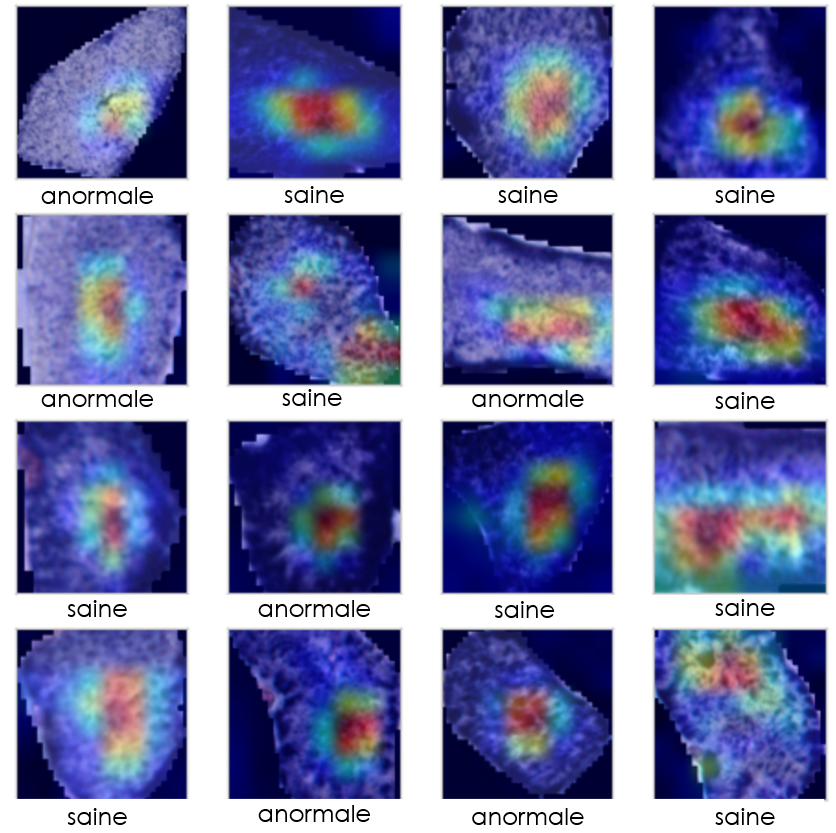
\includegraphics[width=0.8\textwidth]{figures/sdh_gradcam.png}
 \caption[Visualisation par méthode \textit{Grad-Cam} du modèle SDH]{\textbf{Visualisation par méthode \textit{Grad-Cam} de la classification de 16 fibres par le modèle SDH}. Les 16 fibres ont été prises au hasard du jeu de test. Superposition de l'image originale re-dimensionnée et de la carte thermique générée. La couleur rouge indique une importance forte pour la décision de classification par le modèle. Une couleur bleue indique une importance fiable.}
 \label{fig:gradcam_sdh}
\end{figure}
La figure \ref{fig:gradcam_sdh} présente les résultats de cette méthode de visualisation sur 16 fibres musculaires uniques prise au hasard dans le jeu de test. On observe sur cette figure que la zone déterminante (représentée par une couleur rouge) pour la classification des fibres selon le modèle est le centre de la fibre musculaire. Cette observation est cohérente, car nous avons observé que dans la majorité des cas, une fibre est dite anormale lorsqu'elle présente une agglutination de coloration au centre de la fibre (agrégats de mitochondries centralisés). Ce résultat confirme donc que le modèle porte son attention globalement sur la même zone que l'expert lors de la classification manuelle. 

\subsubsection{\textit{Embedding} des images et réduction de dimensionnalité} 
Pour rappel, la notion d'\textit{embedding} correspond à la transformation d'une donnée en un vecteur numérique de grande taille. Dans \gls{nlmyo} nous avons utilisé des techniques d'\textit{embedding} sur des données textuelles. Ici, nous avons réalisé un \textit{embedding} de nos images, non pas pour faire de la classification, mais pour appliquer des techniques de réduction de dimensionnalité pour visualiser si notre modèle est bien capable de faire une différence nette entre les deux classes.

Pour cela, nous avons utilisé notre modèle \gls{sdh} et avons retiré la dernière couche de neurones servant à la classification. Ainsi la sortie du modèle correspond à la sortie de la dernière couche convolutive, c'est-à-dire à un vecteur de taille (1, 2048) correspondant aux caractéristiques importantes de l'image extraite par le modèle pour la classification. En réalisant cette opération pour l'ensemble des images, nous obtenons une matrice (16 787, 2048) sur laquelle nous appliquons une méthode de réduction de dimensionnalité (nommée UMAP (\cite{mcinnes_umap_2020})), donnant ainsi une matrice (16 787, 2) visualisable facilement en deux dimensions.
\begin{figure}[!ht]
 \centering
 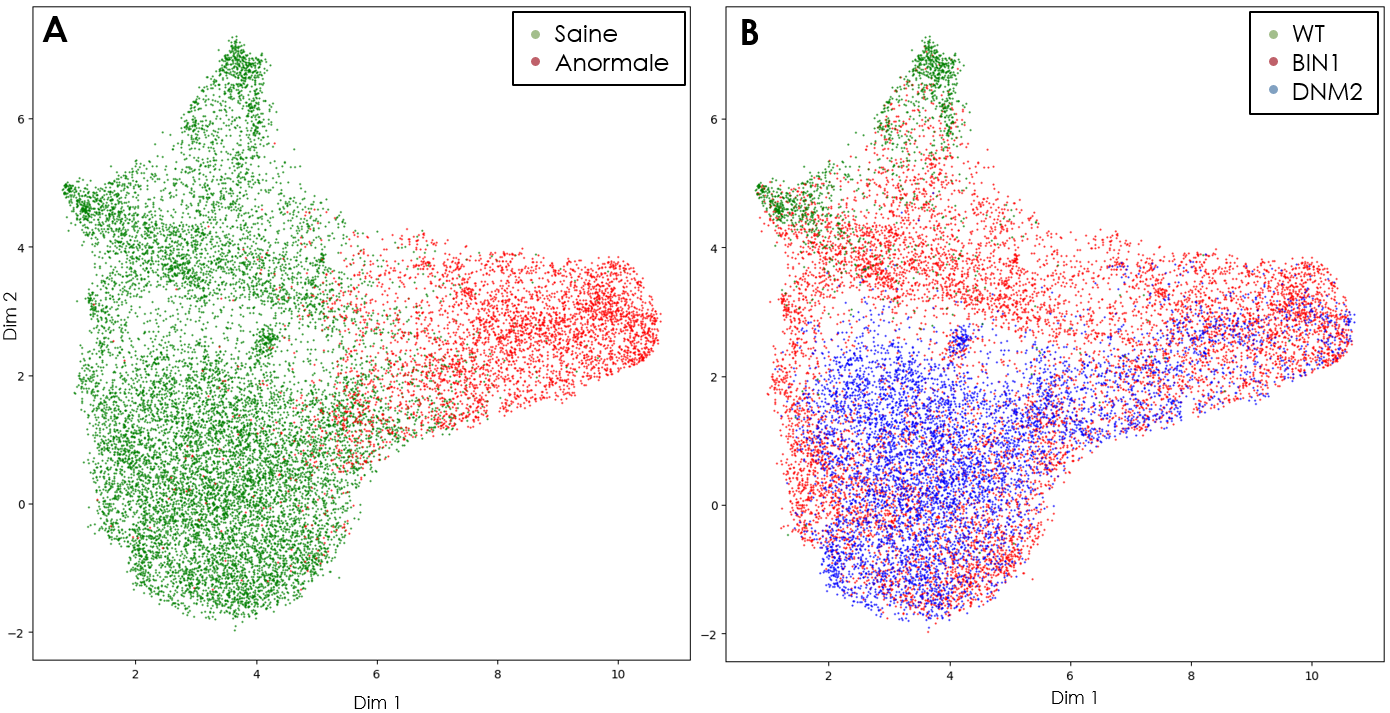
\includegraphics[width=1\textwidth]{figures/umap_sdh.png}
 \caption[Visualisation de l'\textit{embedding} du modèle SDH]{\textbf{Visualisation de l'\textit{embedding} du modèle SDH des 16 787 images de fibres musculaires après réduction de dimensionnalité par UMAP.} \textbf{(A)} Les fibres sont colorées par label (Saine en vert, Anormale en rouge) \textbf{(B)} Les fibres sont colorées par modèle de souris (WT en vert, BIN1 en rouge, DNM2 en bleu).}
 \label{fig:umap_sdh}
\end{figure}

Ainsi, la figure \ref{fig:umap_sdh} présente la visualisation obtenue après \textit{embedding} et réduction de dimensionnalité des 16 787 images du jeu de données. Chaque point représente une image du jeu de données, colorée selon son label (annotation) ou sa provenance (modèle de souris). Globalement on observe que sur le premier (et donc le plus important) axe de variance (en abscisse), le modèle extrait des informations permettant de faire la différence entre les fibres saines et anormales. En effet, les deux classes de fibres sont bien séparées avec cependant la présence d'un continuum entre les deux groupes indiquant la présence de fibres avec des profils intermédiaires plus complexes. Le second axe de variance (en ordonnée) indique que le modèle extrait aussi des informations permettant d'établir la provenance de la fibre, c'est-à-dire de quel modèle de souris elle est issue. En effet, on voit un cluster de fibres venant de souris \textit{wild-type} assez compacte en haut de la figure, puis deux clusters à la fois superposés et séparés de fibres provenant de souris modèle \textit{BIN1} et \textit{DNM2}. L'ensemble des ces résultats confirment que notre modèle extrait et base sa classification des fibres sur les caractéristiques intrinsèques des fibres saines ou anormales et non, sur des biais extérieurs.

\subsubsection{Identification des erreurs d'annotation par le modèle}
Lors de la phase de test, le modèle a obtenu une exactitude de classification de 93.2\%, il existe donc une marge de progression pour le modèle. Les 6.8\% d'erreur peuvent être expliqués par plusieurs raisons. La première est que le modèle n'est peut-être pas assez complexe pour capturer l'ensemble des critères de classification des images et donc a des difficultés pour certains cas complexes. Cependant, cette explication a peu de chance d'être fondée, car nous utilisons une architecture \textit{Resnet50} ayant fait ses preuves dans diverses taches de classification biomédicales avec plus de 25 millions de paramètres, ce qui est suffisant pour détecter une tache centrale sur des images de petite résolution. Un seconde raison expliquant ces erreurs pourrait être la présence de bruit ou d'erreurs dans le jeu de données de base (erreurs d'annotations). Nous avons alors exploré comment nous pouvions, grâce au modèle entrainé, identifier de potentielles erreurs d'annotations dans notre jeu de données.

La figure \ref{fig:identify_errors} résume la démarche utilisée pour identifier des erreurs dans le jeu de données. À partir de la prédiction de la classe des 16 787 images, nous avons filtré pour ne garder que les images où le label (annotation par l'expert) était discordant avec la prédiction du modèle ET où le modèle avait un fort niveau de confiance dans la prédiction (>85\%). Au total, cela représente 228 images, soit 1.66\% du jeu de donnée de base.
\begin{figure}[!ht]
 \centering
 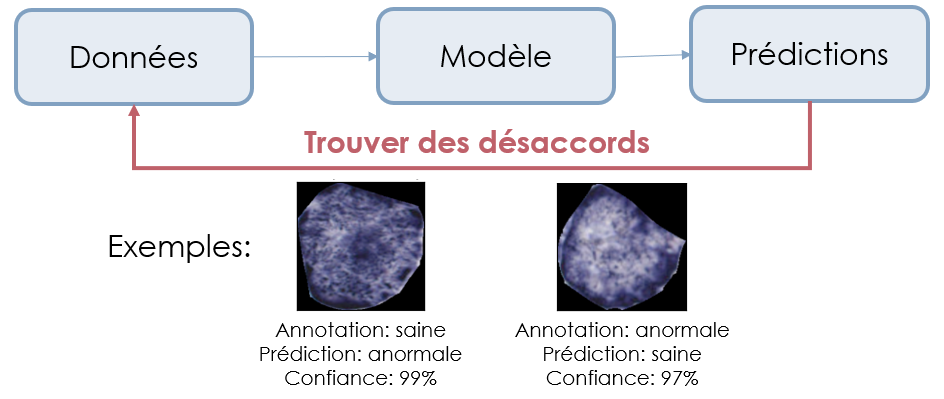
\includegraphics[width=1\textwidth]{figures/identify_errors.png}
 \caption[Méthode d'identification des potentielles erreurs d'annotation]{\textbf{Méthode d'identification des erreurs d'annotation potentielles.} À partir des annotations et des prédictions du modèle sur le jeu de données, nous extrayons les images pour lesquelles le modèle prédit une classe contraire à l'annotation, avec un haut taux de confiance dans la prédiction.}
 \label{fig:identify_errors}
\end{figure}

La figure \ref{fig:list_errors} présente huit exemples pris au hasard parmi les 228 images ayant une prédiction discordante avec l'annotation et un haut niveau de confiance du modèle. On observe par exemple pour la fibre n°1 et la fibre n°8, qu'elles ont été annotées par l'expert comme saines et prédites comme anormales par le modèle. En regardant l'image de la fibre, on observe une tache centrale caractéristique de fibres ayant une répartition mitochondriale anormale. Ceci laisse donc penser qu'il y a eu une erreur d'annotation pour ces deux fibres, considérée à tort comme saine. De même, pour la fibre n°2, annotée comme anormale, mais prédite comme saine, on observe la présence d'un marquage homogène sans agglutination caractéristique du marquage au centre, il n'y a donc visiblement pas de raison pour la classer comme anormale. À l'inverse, pour l'image n°5, annotée comme saine, la prédiction du modèle est "anormale" avec un taux de confiance de 96\%, malgré une apparence sombre, il ne semble pas y avoir de marquage particulièrement prononcé au centre de la fibre comparé à la périphérie, ce qui correspond donc probablement à une vraie erreur du modèle.

Ces résultats montrent que le modèle est capable d'identifier des erreurs humaines lors de l'évaluation des fibres. Ces erreurs d'annotation peuvent être dues à des inattentions ou des erreurs de clic lors du travail manuel et répétitif d'annotation des 16 787 images par les experts. La détection de potentielles erreurs par le modèle et leur ré-annotation pourrait permettre d'améliorer le jeu de données utilisé pour l'entrainement du modèle et ainsi obtenir de meilleures performances de classification.
\begin{figure}[!ht]
 \centering
 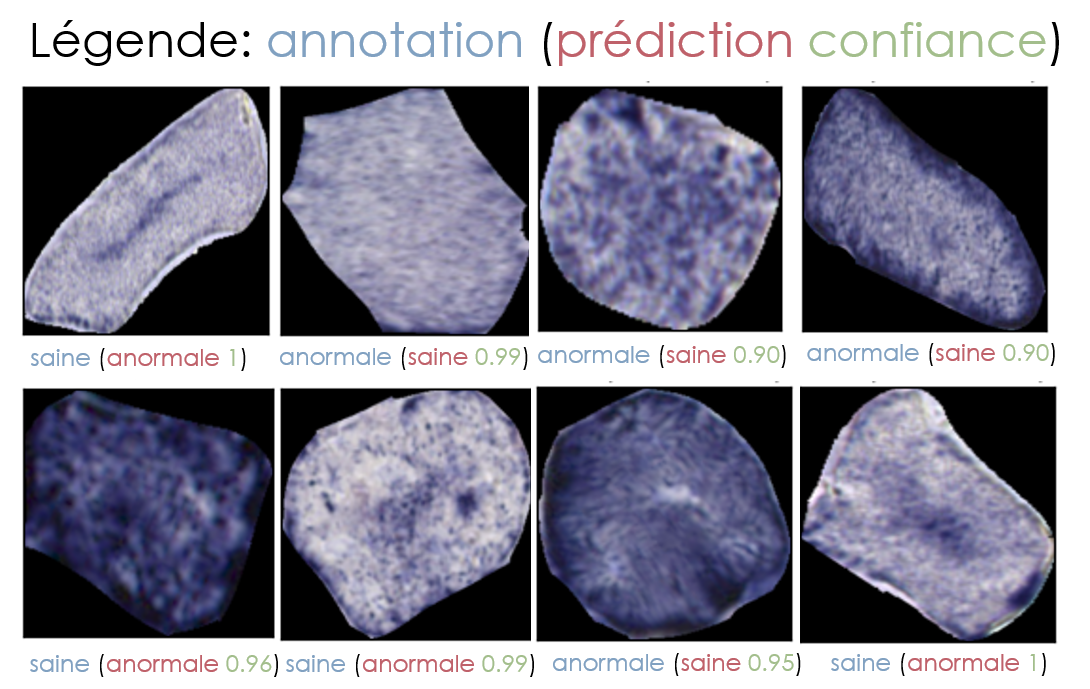
\includegraphics[width=1\textwidth]{figures/list_sdh_errors.png}
 \caption[Exemple de fibres ayant un label prédit contraire a l'annotation avec un haut niveau de confiance du modèle]{\textbf{Exemple de fibres ayant un label prédit contraire à l'annotation avec un haut niveau de confiance du modèle}. L'annotation par l'expert est écrite en bleue, la prédiction du modèle en rouge et sa confiance dans la prédiction en vert (comprise entre 0 et 1). Les fibres n°1, 2 et 8 semblent avoir une mauvaise annotation par l'expert. La fibre n°5 semble être bien annotée et est probablement une erreur réelle du modèle.}
 \label{fig:list_errors}
\end{figure}

\section{Déploiement de la plateforme}
Pour faciliter l'utilisation et la diffusion de \gls{myoquant}, nous avons développé l'outil sous deux formes: un outil en ligne de commande et une version de démonstration en ligne.

\subsection{Outil en ligne de commande}
Sous sa forme d'outil en ligne de commande, \gls{myoquant} est téléchargeable comme bibliothèque Python disponible dans le répertoire officiel PyPI à l'adresse \href{https://pypi.org/project/myoquant/}{https://pypi.org/project/myoquant/}. La version en ligne de commande permet de traiter un grand nombre d'images et/ou des images de coupes complètes trop grandes pour être traitées \textit{via} une interface en ligne. Ceci permet de traiter les images sur des serveurs de calcul équipés de \gls{gpu} afin d'accélérer le processus d'analyse et de sauvegarder l'ensemble des résultats.

\subsection{Version de démonstration en ligne}
\gls{myoquant} est aussi disponible sous forme d'interface de démonstration en ligne développée grâce à \textit{Streamlit}. Cette interface en ligne est utile pour faire des démonstrations de l'outil de façon visuelle, notamment grâce à la génération des différentes figures présentée ci-dessus améliorant l'explicabilité des classifications (analyse de la centralisation pour la coloration HE, histogrammes et courbe de densité pour la coloration ATPase, méthode Gradcam pour le modèle SDH). Cette interface permet aussi de tester l'outil sur des images de petites tailles afin d'évaluer quels seraient les meilleurs paramètres pour obtenir une classification de qualité. \gls{myoquant}-\textit{Streamlit} est disponible en ligne à l'adresse \href{https://lbgi.fr/MyoQuant/}{https://lbgi.fr/MyoQuant/} ainsi que sur \textit{HuggingFace Space} \href{https://huggingface.co/spaces/corentinm7/MyoQuant}{https://huggingface.co/spaces/corentinm7/MyoQuant}.

\section{Limites et perspectives de développement}
L'outil \gls{myoquant} permet de quantifier des marqueurs pathologiques dans trois des cinq colorations réalisées en routine pour le diagnostic des \gls{mc}. Pour l'instant, \gls{myoquant} n'inclus pas de méthode dédiée à l'analyse des coupes à la coloration \gls{tg} pour détecter les agrégats protéiques ni de méthode pour la coloration NADH pouvant mettre en évidence la présence de \textit{cores}. Des modèles \gls{ia} suivant la même méthodologie que ce que nous avons développé pour la coloration \gls{sdh} devront être développés en conséquence. Il est aussi nécessaire pour certaines colorations d'élargir le champ des marqueurs pathologiques quantifiés. Par exemple, pour la coloration \gls{he}, la taille des fibres pour la détection de fibres atrophiques est aussi évaluée en routine lors du diagnostic en complément de la position des noyaux.

De plus, \gls{myoquant} a majoritairement été développé à partir de données issues de biopsies musculaires de souris. Il serait intéressant de tester \gls{myoquant} sur un jeu de données de biopsies humaines quantifiées manuellement par un expert pour évaluer son niveau de performance sur des données humaines. En cas de performance satisfaisante, il serait alors possible d'analyser de façon massive les données de patients afin d'établir de potentiels seuils pour chaque marqueur pathologique pour le diagnostic automatique de \gls{mc}.

 Enfin, sur un plan technique, il serait intéressant de développer une interface en ligne pour \gls{myoquant} liée à des \gls{gpu} pour le traitement de coupes complètes en un temps raisonnable sans avoir à utiliser la ligne de commande, qui est un frein majeur pour un public non expérimenté en programmation, ce qui est typiquement le cas lors du diagnostic.